\documentclass{report} 
\title{Signals And Systems by Alan V. Oppenheim:\\Notes}
\date{Started 17 April 2025}
\author{Malcolm}
\usepackage{amsmath} %import math
\usepackage{mathtools} %more math
\usepackage{amssymb} %for QED symbol
\usepackage{amsthm} %
\usepackage{bm}%bold math
\usepackage{graphicx} %import imaging
\graphicspath{{./images/}} %set imaging path
\begin{document}
\maketitle

\tableofcontents

\newpage
\chapter{Introduction}
\section{Signal Energy and Power}
\textbf{Motivation and definition}\\
In many but not all, applications, the signals considered directly related to physical quantities capturing
power and energy in a physical system. (for instance $v^2/R$ for the power across a resistor)\\
\vspace{1mm}\\
As such it is a common and worthwhile convention to use similar terminology for power and energy for \textit{any} 
continuous-time signal, denoted $x(t)$, or any discrete-time signal $x[n]$. 
In this case, the total energy over the time interval $t_1\leq t\leq t_2$ in a continuous signal $x(t)$ is defined
as
\begin{equation*}
\int^{t_2}_{t_1}|x(t)|^2dt
\end{equation*}
where $|x|$ denotes the magnitude of the (possibly complex) number $x$; see that the time-averaged signal 
can be obtained by dividing by $(t_2-t_1)$. Similarly for a discrete signal $x[n]$ over the interval $n_1\leq n\leq n_2$ the total energy is
\begin{equation*}
\sum^{n_2}_{n=n_1}|x[n]|^2
\end{equation*}
with the average power calculated by dividing by $(n_2-n_1+1)$.\\
\vspace{1mm}\\
It is important to remember that the terms `power' and `energy' are used here \textit{independently} of their 
relation to physical energy (they clearly don't correlate since their units or scalings would differ). Nevertheless
we will find it convenient to use these terms in a general fashion.\\
\vspace{1mm}\\
\textbf{Power and energy over infinite intervals}\\
Considering signals over an infinite time interval, meaning for $-\infty<t<+\infty$ or $-\infty<n<+\infty$. 
Here we define the total energy as the limits of the aforementioned equations increase without bound; in continuous
time,
\begin{equation*}
E_\infty\triangleq\lim_{T\to\infty}\int^T_{-T}|x(t)|^2dt
=\int^{+\infty}_{-\infty}|x(t)|^2dt
\end{equation*}
and in discrete time,
\begin{equation*}
E_\infty\triangleq\lim_{N\to\infty}\sum^{+N}_{n=-N}|x[n]|^2=\sum^{+\infty}_{n=-\infty}|x[n]|^2
\end{equation*}
Note that these expressions may not converge; for instance say $x(t)$ or $x[n]$ equal some nonzero constant for 
all time: such signals have infinite energy, while signals with $E_\infty<\infty$ have finite energy.\\
(next page)\newpage
\noindent\textbf{Cont.}\\
Analagously, we can define the time-averaged power over an infinite interval as
\begin{equation*}
P_\infty\triangleq\lim_{T\to\infty}\frac{1}{2T}\int^T_{-T}|x(t)|^2dt
\end{equation*}
and
\begin{equation*}
P_\infty\triangleq\lim_{N\to\infty}\frac{1}{2N+1}\sum^{+N}_{n=-N}|x[n]|^2
\end{equation*}
In continuous and discrete time respectively. \\
\vspace{1mm}\\
\textbf{Intuition}\\
See that with these definitions, we can identify three classes of signals: first those with finite total energy,
meaning $E_\infty<\infty$. See that such a signal would have zero average power:
\begin{equation*}
P_\infty=\lim_{T\to\infty}\frac{E_\infty}{2T}=0
\end{equation*}
Second would be signals with finite average power $P_\infty$; see from the above expression that for $P_\infty>0$,
this requires that $E_\infty=\infty$.\\
\vspace{1mm}\\
Last would be signals for which neither $P_\infty$ nor $E_\infty$ are finite. An example of this might be $x(t)=t$.\\
\vspace{1mm}\\
\textbf{Note on discrete signals}\\
It is important to note that the discrete-time signal $x[n]$ is defined \textit{only} for \textit{integer} 
values of the independent variable.
\newpage

\section{Even and Odd signals}
\textbf{Definition}\\
A continuous-time signal is \textit{even} if
\begin{equation*}
x(-t)=x(t)
\end{equation*}
while a discrete-time signal is \textit{even} if
\begin{equation*}
x[-n]=x[n]
\end{equation*}
These signals are referred to as \textit{odd} if
\begin{align*}
x(-t)&=-x(t)\\
x[-n]&=-x[n]
\end{align*}
Note that an odd signal must be 0 at $t=0$ or $n=0$ since the equations require that $x(0)=-x(0)$ and $x[0]=-x[0]$.
\\
\vspace{1mm}\\
\textbf{Decomposition}\\
An important fact is that any signal can be broken into a sum of two signals, where one is even and the other odd.
To see this, consider
\begin{equation*}
\text{Ev}\{x(t)\}=\frac{1}{2}[x(t)+x(-t)]
\end{equation*}
which is referred to as the \textit{even part} of $x(t)$. Similarly, the \textit{odd part} of $x(t)$ is given by
\begin{equation*}
\text{Od}\{x(t)\}=\frac{1}{2}[x(t)-x(-t)]
\end{equation*}
See that $x(t)$ is the sum of the two. Exactly analagous definitions hold in the discrete time case.
\begin{center}
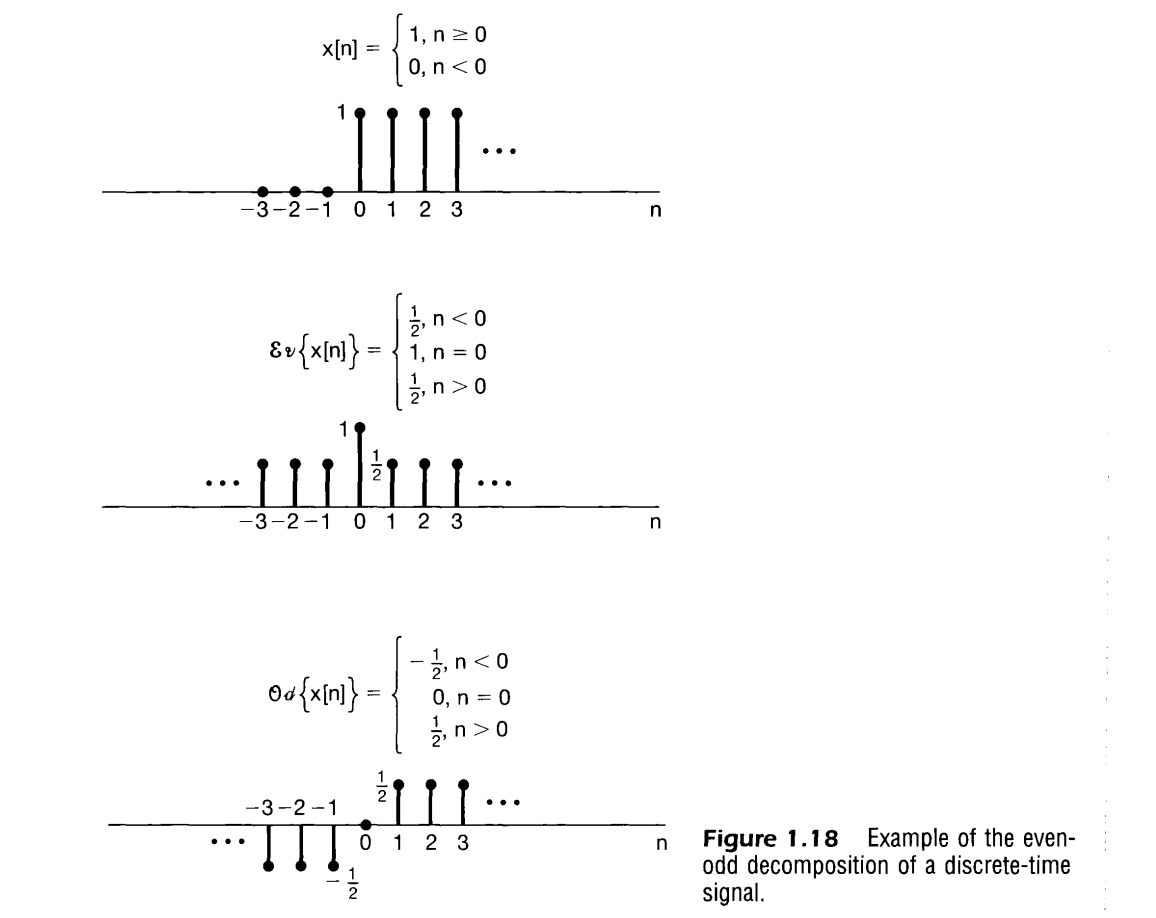
\includegraphics[width=9cm]{a1}
\end{center}
\newpage

\section{Differences between continuous and\\discrete periodic complex exponentials}
The continuous-time \textit{complex exponential signal} is of the form
\begin{equation*}
x(t)=Ce^{at}
\end{equation*}
where $C$ and $a$ are, in general, complex numbers. An important class of complex exponentials is obtained by constraining $a$ to be purely imaginary:
\begin{equation*}
x(t)=e^{i\omega t}
\end{equation*}
\textbf{Periodicity and harmonic relations (purely imaginary power)}\\
An important property of this signal is that it is periodic; recall that $x(t)$ will be periodic with period $T$ if
\begin{equation*}
e^{i\omega t}=e^{i\omega(t+T)}
\end{equation*}
this means
\begin{equation*}
e^{i\omega(t+T)}=e^{i\omega t}e^{i\omega T}\implies
e^{i\omega T}=1
\end{equation*}
If $\omega=0$ then this is satisfied for any $T$. If $\omega\neq0$, see that the \textit{fundamental period} 
$T_0$ of $x(t)$---that is, the smallest positive value of $T$ for which this holds---is
\begin{equation*}
T_0=\frac{2\pi}{|\omega|}
\end{equation*}
(the signals $e^{i\omega 0t}$ and $e^{-i\omega t}$ have the same fundamental period)
Naturally, there is a set of exponentials periodic to a common period $T_0$. These are said to be
\textit{harmonically related} complex exponentials; the necessary condition they satisfy is
\begin{equation*}
e^{i\omega T_0}=1
\end{equation*}
which implies that
\begin{equation*}
\omega T_0=2\pi k,\quad k=0,\pm1,\pm2,\ldots
\end{equation*}
(next page)\newpage
\noindent\textbf{Cont.}\\
We had
\begin{equation*}
\omega T_0=2\pi k,\quad k=0,\pm1,\pm2,\ldots
\end{equation*}
if we define
\begin{equation*}
\omega_0=\frac{2\pi}{T_0}
\end{equation*}
this means that the harmonic frequencies $\omega$ must be integer multiples of $\omega_0$:
\begin{equation*}
\phi_k(t)=e^{ik\omega_0t},\quad k=0,\pm1,\pm2,\ldots
\end{equation*}
For $k=0$, $\phi_k(t)$ is a constant, while for any other value of $k$, $\phi_k(t)$ is periodic with fundamental 
frequency $|k|\omega_0$ and fundamental period
\begin{equation*}
\frac{2\pi}{|k|\omega_0}=\frac{T_0}{|k|}
\end{equation*}
Each $\phi_k(t)$ itself defines a fundamental frequency and a corresponding fundamental period. 
(see that $|k|\omega_0\cdot T_0/|k|=2\pi$, so this scaled down period is the corresponding period
for this scaled up frequency. Each frequency is unique, point here is that they are also periodic with $T_0$, 
but with fundamental periods getting proportionally smaller.)\\
\vspace{1mm}\\
Note that the $k$th harmonic $\phi_k(t)$ is still periodic with $T_0$; it goes through exactly $|k|$ of its 
fundamental periods during any time interval of length $T_0$. (the term `harmonic' is consistent with its use in
music, where it refers to tones resulting from variations in acoustic pressure at frequencies that are integer
multiples of a fundamental frequency)\\
(next page)\newpage
\noindent\textbf{Discrete case}\\
As in continuous time, an important signal in discrete time is the \textit{complex exponential signal}, defined as
\begin{equation*}
x[n]=C\alpha^n
\end{equation*}
where $C$ and $\alpha$ are, in general, complex numbers. See that this could also be expressed as
\begin{equation*}
x[n]=Ce^{\beta n}
\end{equation*}
where $\alpha=e^\beta$. See that we can constrain $\beta$ to be purely imaginary:
\begin{equation*}
x[n]=e^{i\omega_0n}
\end{equation*}
\textbf{Periodicity properties of Discrete-time complex exponentials}\\
While there are many similarities between continuous and discrete-time signals, there are a number of important
differences. For the continuous time signal $e^{i\omega_0t}$, we know that
\begin{itemize}
\item The larger the magnitude of $\omega_0$, the higher the rate of oscillation of the signal
\item $e^{i\omega_0t}$ is periodic for any value of $\omega_0$
\end{itemize}
These properties are different in the discrete-time case.\\
\vspace{1mm}\\
Given the first property, consider the discrete-time complex exponential with frequency $\omega_0+2\pi$:
\begin{equation*}
e^{i(\omega_0+2\pi)n}=e^{i2\pi n}e^{i\omega_0n}=e^{i\omega_0n}
\end{equation*}
(see that this is a direct result of the fact that we iterate through discrete time as integers) 
The exponential at frequency $\omega_0+2\pi$ is the \textit{same} as that at frequency $\omega_0$. 
This is unlike the continuous-time case where each distinct $\omega_0$ represents a distinct signal.\\
\vspace{1mm}\\
In discrete time, the signal with frequency $\omega_0$ is identical to the signals with frequencies 
$\omega_0\pm2\pi,\omega_0\pm4\pi$, and so on. Therefore when considering discrete time complex exponentials, 
see that we need only consider a frequency interval of length $2\pi$ in which to choose $\omega_0$, such as 
$0\leq\omega_0<2\pi$ or $-\pi\leq\omega_0<\pi$.\\
\vspace{1mm}\\
Also see that because of this the discrete exponential 
$e^{i\omega_0n}$ does \textit{not} have a continually 
increasing rate of oscillation as $\omega_0$ increases in magnitude; the signals will oscillate faster until we 
reach $\omega_0=\pi$, after which the rate of oscillation decreases until we reach $\omega_0=2\pi$, at which 
the same constant sequence as $\omega_0=0$ is produced.\\
(next page)\newpage
\noindent\textbf{Cont.}\\
The second property we wish to consider concerns the periodicity of the discrete time complex exponential. In
order for the signal $e^{i\omega_0n}$ to be periodic with
period $N>0$ we must have
\begin{equation*}
e^{i\omega_0(n+N)}=e^{i\omega_0n}
\end{equation*}
or equivalently 
\begin{equation*}
e^{i\omega_0N}=1
\end{equation*}
For this to hold, $\omega_0N$ must be a multiple of $2\pi$. That is, there must be an integer $m$ such that
\begin{equation*}
\omega_0N=2\pi m
\end{equation*}
or equivalently
\begin{equation*}
\frac{\omega_0}{2\pi}=\frac{m}{N}
\end{equation*}
The signal $e^{i\omega_0n}$ is periodic if $\omega_0/2\pi$ is a rational number and is not periodic otherwise.\\
\vspace{1mm}\\
\textbf{Fundamental period}\\
Recall the idea of a \textit{fundamental period}; in this case it would mean the smallest $N$ such that 
$\omega_0N=2\pi m$ holds (this is unlike the continuous case where there is always some $T$ where $\omega_0T=2\pi$); see that this occurs when $m$ and $N$ do not have any factors in common.\\
\vspace{1mm}\\
See that from this we can derive a \textit{fundamental frequency} as
\begin{equation*}
\frac{2\pi}{N}=\frac{\omega_0}{m}
\end{equation*}
(see that this frequency is always equal or lower---intuitively, to have a different wave that completes one
oscillation in $N$ time, its frequency will either be equal or lower)\\
\vspace{1mm}\\
To summarize
\begin{center}
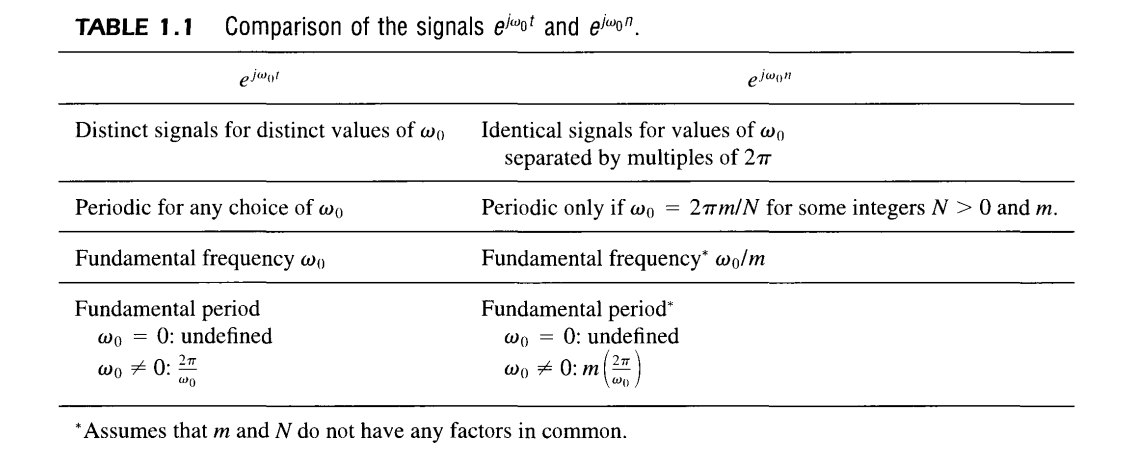
\includegraphics[width=10cm]{a2}
\end{center}
\newpage

\section{Intuition for discrete-time periodicity}
Consider the sequence $x[n]=\cos(2\pi n/12)$:
\begin{center}
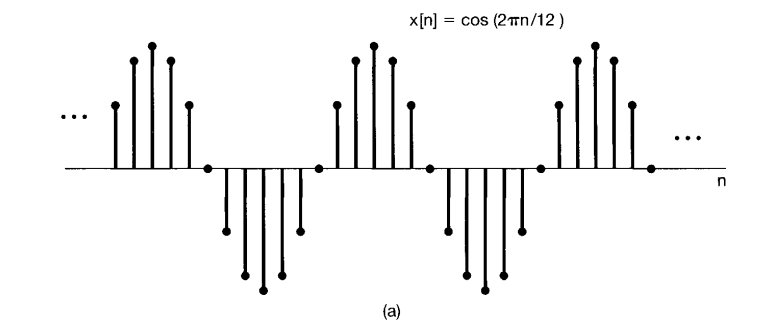
\includegraphics[width=10cm]{a3}
\end{center}
we can think of this as a set of samples of the continuous-time sinusoid $x(t)=\cos(2\pi t/12)$ at integer time
points. In this case, see that both $x(t)$ and $x[n]$ are periodic with fundamental period 12.
That is, the values of $x[n]$ repeat every 12 points, exactly in step with the fundamental period of $x(t)$.\\
\vspace{1mm}\\
Now consider the signal $x[n]=\cos(8\pi n/31)$:
\begin{center}
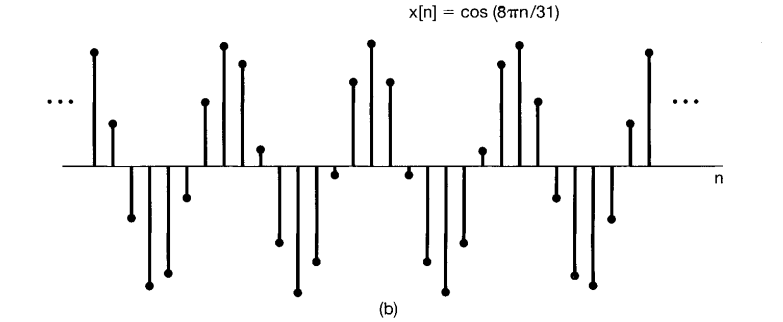
\includegraphics[width=10cm]{a4}
\end{center}
This can also be viewed as a set of samples of $x(t)=\cos(8\pi t/31)$ at integer points in time. 
But now see that in this case $x(t)$ is periodic with fundamental period $31/4$, while $x[n]$ is periodic with 
fundamental period 31.\\
\vspace{1mm}\\
This difference stems from the fact that the discrete-time signal is defined only for integer values of the 
independent variable---there is no sample at time
$t=31/4$, when $x(t)$ completes one period, or at $t=2\cdot31/4$ or $t=3\cdot31/4$, when $x(t)$ has completed two
or three periods. Only at sample $t=4\cdot31/4=31$, when
$x(t)$ has completed \textit{four} periods is the discrete sequence defined.\\
\vspace{1mm}\\
This manifests as the pattern of $x[n]$ not repeating with each cycle of positive and negative values, but rather
only after four of such cycles, specifically 31 points.\\
(next page)\newpage
\noindent\textbf{Cont.}\\
Finally consider the signal $x[n]=\cos(n/6)$:
\begin{center}
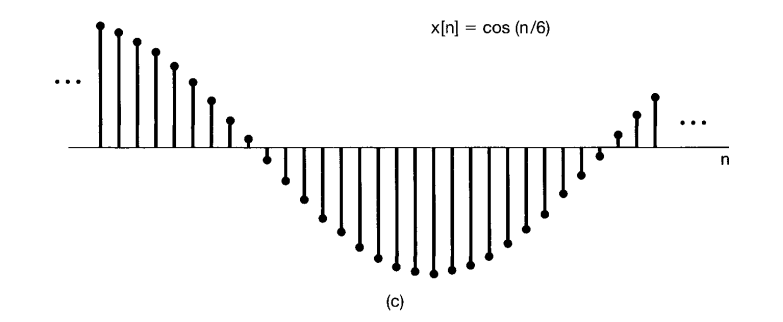
\includegraphics[width=10cm]{a5}
\end{center}
In this case, the values of $x(t)$ at integer sample points \textit{never repeat}, as these sample points never
span an interval that is an exact multiple of the period,
$12\pi$, of $x(t)$.\\
\vspace{1mm}\\
Thus, $x[n]$ \textit{is not periodic}, although the eye visually interpolates between the sample points,
suggesting \textit{the envelope} $x(t)$ which is periodic.
\newpage

\section{Difference in harmonic relations in discrete and\\continuous periodic exponentials}
As in continuous time, it is also of considerable value in discrete-time to consider sets of harmonically related
periodic exponentials---that is, \textit{periodic exponentials with a common period $N$}.\\
\vspace{1mm}\\
We know that these are precisely the signals which are at frequencies which are multiples of $2\pi/N$; that is
\begin{equation*}
\phi_k[n]=e^{ik(2\pi/N)n},\quad k=0,\pm1,\ldots
\end{equation*}
In the continuous-time case, all the harmonically related complex exponentials 
$e^{ik(2\pi/T_0)t},\,k=0,\pm1,\pm2,\ldots$ are distinct.
However, recall that for discrete signals we have
\begin{equation*}
e^{i(\omega_0+2\pi)n}=e^{i2\pi n}e^{i\omega_0n}=e^{i\omega_0n}
\end{equation*}
(this is a direct result of the fact that we iterate through discrete time as integers) As such the harmonically
related complex exponentials \textit{are not all unique in discrete time}; specifically,
\begin{align*}
\phi_{k+N}[n]&=e^{i(k+N)(2\pi/N)n}\\
&=e^{ik(2\pi/N)n}e^{i2\pi n}=\phi_k[n]
\end{align*}
See that this implies that there are only $N$ distinct 
periodic exponentials in the set of $\phi_k[n]$; meaning
\begin{equation*}
\phi_0[n]=1,\,\phi_1[n]=e^{i(2\pi/N)n},\,
\phi_2[n]=e^{i2(2\pi/N)n},\ldots,\,
\phi_{N-1}[n]=e^{i(N-1)(2\pi/N)n}
\end{equation*}
are all distinct, but any other $\phi_k[n]$ would just be identical to one of them. (for instance $\phi_N[n]=\phi_0[n]$ or $\phi_{-1}[n]=\phi_{N-1}[n]$.)
\newpage

\section{More on complex exponential and sinusoidal signals}
\textbf{Continuous case}\\
A continuous-time \textit{complex exponential signal} is of the form 
\begin{equation*}
x(t)=Ce^{at}
\end{equation*}
where $C$ and $a$ are, in general, complex numbers.\\
\vspace{1mm}\\
\textbf{Euler identity and `combined' sinusoidal form}\\
Recall euler's identity:
\begin{equation*}
e^{i\omega_0t}=\cos(\omega_0t)+i\sin(\omega_0t)
\end{equation*}
See that the scaled and phase-delayed sinusoid can be written in terms of these periodic complex exponentials
with the same fundamental period:
\begin{equation*}
A\cos(\omega_0t+\phi)=\frac{A}{2}e^{i\phi}e^{i\omega_0t}
+\frac{A}{2}e^{-i\phi}e^{-i\omega_0t}
\end{equation*}
We can also express
\begin{equation*}
A\cos(\omega_0t+\phi)=A\text{Re}\{e^{i(\omega_0t+\phi)}\}
\end{equation*}
and
\begin{equation*}
A\sin(\omega_0t+\phi)=A\text{Im}\{e^{i(\omega_0t+\phi)}\}
\end{equation*}
\textbf{Energy and power}\\
Periodic signals---and in particular, the complex periodic exponential signal---are examples of signals
with infinite total energy but finite average power. 
Calculating the total energy and of the periodic exponential signal over one period:
\begin{align*}
E_{\text{period}}&=\int^{T_0}_0|e^{i\omega_0t}|^2dt\\
&=\int^{T_0}_01\,dt=T_0
\end{align*}
(The absolute value of a complex number is its magnitude. Think of the absolute value as the 
(possibly multidimensional) distance from zero.) Calculating the average power:
\begin{equation*}
P_{\text{period}}=\frac{1}{T_0}E_{\text{period}}=1
\end{equation*}
Since there are an infinite number of periods as $t$ ranges from $-\infty$ to $+\infty$, the total energy 
integrated over all time is infinite.
However, since the average power over each period is 1, averaging over multiple periods always yields an average
power of 1. That is, the complex periodic exponential
signal has finite average power equal to
\begin{equation*}
P_\infty=\lim_{T\to\infty}\frac{1}{2T}\int^T_{-T}|e^{i\omega_0t}|^2dt=1
\end{equation*}
(next page)\newpage
\noindent\textbf{General continuous complex exponential signals}\\
In the most general case $Ce^{at}$ where both $C$ and $a$ are complex, see that since $C$ and $a$ can are just
\begin{equation*}
C=|C|e^{i\theta},\quad a=r+i\omega_0
\end{equation*}
we can express the general complex signal as
\begin{equation*}
Ce^{at}=|C|e^{i\theta}e^{(r+i\omega_0)t}=|C|e^{rt}e^{i(\omega_0t+\theta)}
\end{equation*}
we can expand this further as
\begin{equation*}
Ce^{at}=|C|e^{rt}\cos(\omega_0t+\theta)+i|C|e^{rt}\sin(\omega_0t+\theta)
\end{equation*}
\textbf{Discrete case}\\
As in continuous time, the discrete time \textit{complex exponential signal} is defined by
\begin{equation*}
x[n]=C\alpha^n
\end{equation*}
where $C$ and $\alpha$ are, in general, complex numbers. This could alternatively be expressed in the form
\begin{equation*}
x[n]=Ce^{\beta n}
\end{equation*}
where $\alpha=e^{\beta}$.\\
\vspace{1mm}\\
\textbf{Euler identity and `combined' sinusoidal form}\\
As with the continuous case, constraining $\beta$ to be
purely imaginary, we have euler's identity
\begin{equation*}
e^{i\omega_0n}=\cos\omega_0n+i\sin\omega_0n
\end{equation*}
and 
\begin{equation*}
A\cos(\omega_0n+\phi)=\frac{A}{2}e^{i\phi}e^{i\omega_0n}+
\frac{A}{2}e^{-i\phi}e^{-i\omega_0n}
\end{equation*}
\textbf{General discrete complex exponential signals}\\
As with the continuous case, for complex $C$ and $\alpha$, we have
\begin{equation*}
C=|C|e^{i\theta},\quad\alpha=|\alpha|e^{i\omega_0}
\end{equation*}
so the general complex exponential signal can be expressed as
\begin{equation*}
C\alpha^n=|C||\alpha|^n\cos(\omega_0n+\theta)
+i|C||\alpha|^n\sin(\omega_0n+\theta)
\end{equation*}
\newpage

\section{Unit impulse and Unit step functions}
\textbf{Discrete-Time}\\
One of the simplest discrete-time signals is the \textit{unit impulse}/\textit{unit sample}, defined as
\begin{equation*}
\delta[n]=\begin{cases}0,&n\neq0\\
1,&n=0\end{cases}
\end{equation*}
\begin{center}
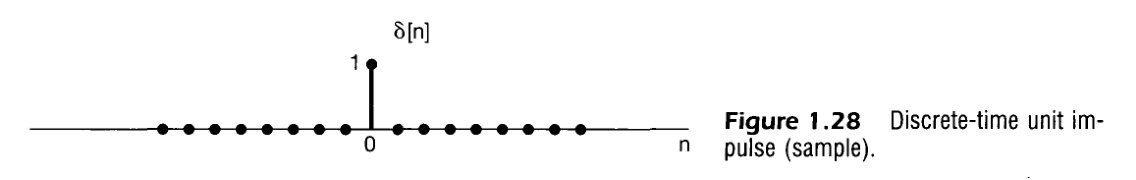
\includegraphics[width=10cm]{a6}
\end{center}
Another basic discrete-time signal is the discrete-time \textit{unit step}, denoted by $u[n]$ and defined by
\begin{equation*}
u[n]=\begin{cases}
0,&n<0\\
1,&n\geq0\end{cases}
\end{equation*}
\begin{center}
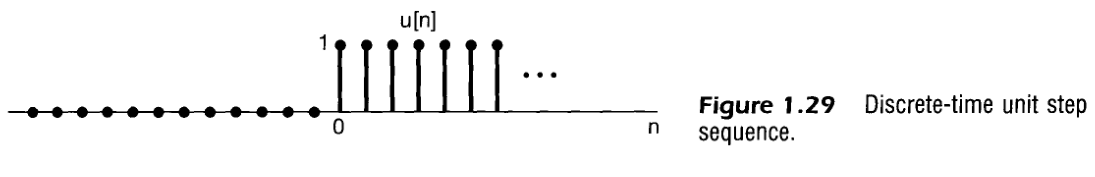
\includegraphics[width=10cm]{a7}
\end{center}
See that the discrete-time unit impulse is the \textit{first difference} of the discrete-time step:
\begin{equation*}
\delta[n]=u[n]-u[n-1]
\end{equation*}
Conversely, the discrete-time unit step is the \textit{running sum} of the unit sample:
\begin{equation*}
u[n]=\sum^n_{m=-\infty}\delta[m]
\end{equation*}
\begin{center}
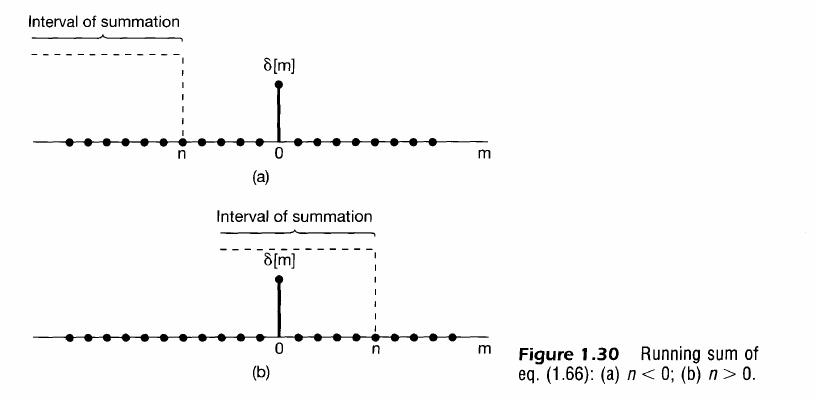
\includegraphics[width=10cm]{a8}
\end{center}
Since the only nonzero value of the unit sample is at 0, the running sum is 0 for $n<0$ and 1 for $n\geq0$.\\
(next page)\newpage
\noindent\textbf{Alternative form}\\
we had the discrete-time unit step as the running sum of the unit sample:
\begin{equation*}
u[n]=\sum^n_{m=-\infty}\delta[m]
\end{equation*}
See that by changing the variable of summation from $m$ to $k=n-m$, we can rewrite this as
\begin{equation*}
u[n]=\sum^0_{k=\infty}\delta[n-k]
\end{equation*}
and equivalently
\begin{equation*}
u[n]=\sum^\infty_{k=0}\delta[n-k]
\end{equation*}
An interpretation of this is a superposition of delayed impulses; we can view the unit step as the sum of unit impulses $\delta[n]$
(nonzero at $n=0$), $\delta[n-1]$ (nonzero at $n=1$), and all other $\delta[n-k]$ for integer $k$ extending to infinity.\\
\vspace{1mm}\\
\textbf{Sampling property}\\
See that the unit impulse can also be used to sample the value of a signal at $n=0$; since $\delta[n]$ is nonzero (and equal to 1)
only for $n=0$, it follows that
\begin{equation*}
x[n]\delta[n]=x[0]\delta[n]
\end{equation*}
More generally, if we consider a unit impulse $\delta[n-n_0]$ at $n=n_0$, then
\begin{equation*}
x[n]\delta[n-n_0]=x[n_0]\delta[n-n_0]
\end{equation*}
(next page)\newpage
\noindent\textbf{Continuous-Time}\\
The continuous-time \textit{unit step function} $u(t)$ is defined in a similar manner to its discrete-time counterpart:
\begin{equation*}
u(t)=\begin{cases}0,&t<0\\
1,&t>0\end{cases}
\end{equation*}
\begin{center}
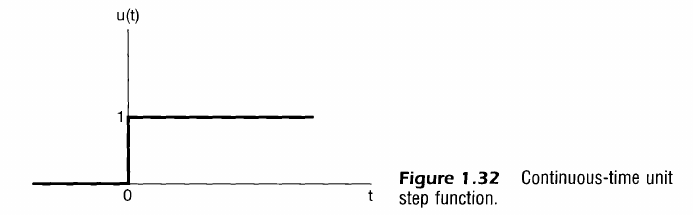
\includegraphics[width=10cm]{a9}
\end{center}
Note that the unit step is \textit{discontinuous} at $t=0$. The continuous-time \textit{unit inpulse} $\delta(t)$ is related to the
unit step in a manner analagous to that of their discrete counterparts; in particular, the continuous-time unit step is the
\textit{running integral} of the unit impulse:
\begin{equation*}
u(t)=\int^t_{-\infty}\delta(\tau)d\tau
\end{equation*}
It also follows that the continuous-time unit impulse can be thought of as the \textit{first derivative} of the continuous-time unit step:
\begin{equation*}
\delta(t)=\frac{du(t)}{dt}
\end{equation*}
In contrast to discrete-time, there is some formal difficulty with this equation as a representation of the unit impulse---since $u(t)$ is 
discontinuous at $t=0$ and consequently is not formally differentiable.\\
(next page)\newpage 
\noindent\textbf{Cont.}\\
We get around this by considering an approximation to the unit step
$u_\Delta(t)$, rising from the value 0 to 1 in a short time interval of
length $\Delta$:
\begin{center}
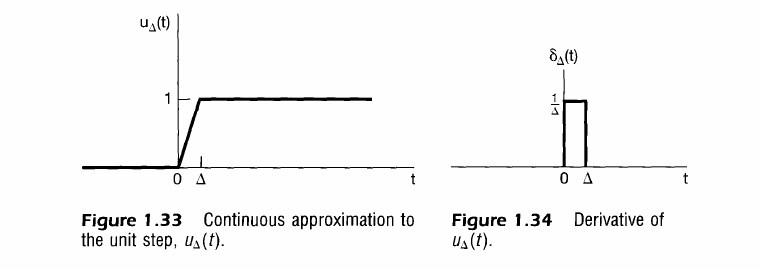
\includegraphics[width=10cm]{a10}
\end{center}
Also considering the derivative:
\begin{equation*}
\delta_\Delta(t)=\frac{du_\Delta(t)}{dt}
\end{equation*}
The unit step changes from value 0 to 1 instantaneously and can be thought of an idealisation of $u_\Delta(t)$ for $\Delta$ so short
that its duration doesn't matter for any practical purpose.
Formally, $u(t)$ is the limit of $u_\Delta(t)$ as $\Delta\to0$.\\
\vspace{1mm}\\
Consider the derivative again; $\delta_\Delta(t)$ is a short pulse, of duration $\Delta$ and unit area for any value of $\Delta$.
As $\Delta\to0$, $\delta_\Delta(t)$ becomes narrower and higher while mantaining its unit area. Its limiting form
\begin{equation*}
\delta(t)=\lim_{\Delta\to0}\delta_\Delta(t)
\end{equation*}
can then be thought of as an idealisation of the short pulse $\delta_\Delta(t)$ as the duration $\Delta$ becomes insignificant:
\begin{center}
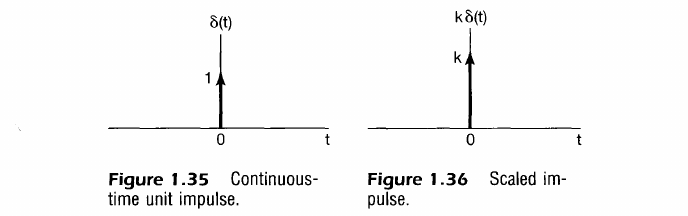
\includegraphics[width=10cm]{a11}
\end{center}
$\delta(t)$ has, in effect, no duration but unit area. The arrow at $t=0$ indicates the area of the pulse is concentrated
at $t=0$ and the height of the arrow and the `1' next to the arrow is used to represent the \textit{area} of the impulse. More generally, 
a scaled impulse $k\delta(t)$ will have an area $k$, and thus
\begin{equation*}
ku(t)=\int^t_{-\infty}k\delta(\tau)d\tau
\end{equation*}
A scaled impulse, where the height of the arrow is chosen to be proportional to the area of the impulse.\\
(next page)\newpage
\noindent\textbf{Alternative form}\\
As with discrete time, the relationship between the continuous time unit step and impulse can be rewritten in a different form, 
by changing the variable of integration from $\tau$ to $\sigma=t-\tau$:
\begin{equation*}
u(t)=\int_{-\infty}^t\delta(\tau)d\tau=\int^0_\infty\delta(t-\sigma)(-d\sigma)
\end{equation*}
or equivalently
\begin{equation*}
u(t)=\int_0^\infty\delta(t-\sigma)\,d\sigma
\end{equation*}
(This negation after inverstion of the limits of the integral can be derived from the first fundamental theorem. For a 
more intuitive understanding, consult the definition of the Riemann sum:
\begin{equation*}
\sum^{n-1}_{i=0}f(t_i)(x_{i+1}-x_{i})
\end{equation*}
Considering the $d\tau$, or respectively $d\sigma$, as the width of the step between two argumentsof the sum, if we change the
direction in which we integrate, the step also changes its sign.
In the discrete sum, the summands are not multiplied by this step.)\\
\vspace{1mm}\\
\textbf{Sampling property}\\
As with discrete-time, the continuous-time impulse has a very important sampling property; consider 
\begin{equation*}
x_1(t)=x(t)\delta_\Delta(t)
\end{equation*}
By construction, $x_1(t)$ is zero outside the interval $0\leq t\leq\Delta$. See that for $\Delta$ sufficiently small so that
$x(t)$ is approximately constant over this integral:
\begin{center}
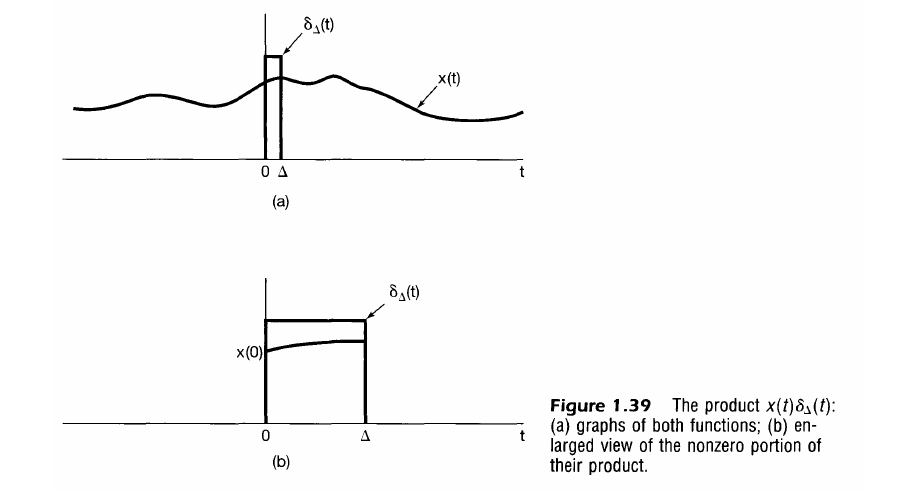
\includegraphics[width=10cm]{a12}
\end{center}
so we have
\begin{equation*}
x(t)\delta_\Delta(t)\approx x(0)\delta_\Delta(t)
\end{equation*}
(next page)\newpage
\noindent\textbf{Cont.}\\
We had, for small $\Delta$,
\begin{equation*}
x(t)\delta_\Delta(t)\approx x(0)\delta_\Delta(t)
\end{equation*}
since $\delta(t)$ is the limit as $\Delta\to0$ of $\delta_\Delta(t)$, it follows that
\begin{equation*}
x(t)\delta(t)=x(0)\delta(t)
\end{equation*}
By the same argument, we have an analagous expression for an impulse concentrated at an arbritrary point, say $t_0$. That is,
\begin{equation*}
x(t)\delta(t-t_0)=x(t_0)\delta(t-t_0)
\end{equation*}
\newpage

\section{Basic system properties 1}
\textbf{General form}\\
A general formula for a continuous first-order linear differential equation is
\begin{equation*}
\frac{dy(t)}{dt}+ay(t)=bx(t)
\end{equation*}
where $x(t)$ is the input, $y(t)$ the output, and $a,b$ constants. An example of this might be
\begin{equation*}
\frac{dv(t)}{dt}+\frac{\rho}{m}v(t)=\frac{1}{m}f(t)
\end{equation*}
Discrete cases have general first-order linear difference equations of the form
\begin{equation*}
y[n]+ay[n-1]=bx[n]
\end{equation*}
Considering the earlier example, if we let $v[n]=v(n\Delta)$ and $f[n]=f(n\Delta)$ and approximate $dv(t)/dt$ at $t=n\Delta$ by
the first backward difference:
\begin{equation*}
\frac{v(n\Delta)-v((n-1)\Delta)}{\Delta}
\end{equation*}
we can obtain
\begin{align*}
\frac{v[n]-v[n-1]}{\Delta}+\frac{\rho}{m}v[n]&=\frac{1}{m}f[n]\\
v[n]-v[n-1]+\frac{\rho\Delta}{m}v[n]&=\frac{\Delta}{m}f[n]\\
v[n]\left(1+\frac{\rho\Delta}{m}\right)-v[n-1]&=\frac{\Delta}{m}f[n]\\
v[n]\frac{m+\rho\Delta}{m}-v[n-1]&=\frac{\Delta}{m}f[n]\\
v[n]-\frac{m}{m+\rho\Delta}v[n-1]&=\frac{\Delta}{m+\rho\Delta}f[n]
\end{align*}
which is in the general form as described above.\\
(next page)\newpage
\noindent\textbf{Basic system properties}\\
\vspace{1mm}\\
\textbf{Memory}\\
A system is said to be \textit{memoryless} if its output for each value of the independent variable is dependent
only on the \textit{input at that same time}.\\
\vspace{1mm}\\
For instance, the system 
\begin{equation*}
y[n]=(2x[n]-x^2[n])^2
\end{equation*}
is memoryless, since the value of $y[n]$ at any particular time $n_0$ depends only on the value of $x[n]$ at that time. 
Other examples of memoryless systems include the input-output relationship of a resistor, with input $x(t)$ taken to be 
current and output $y(t)$ voltage:
\begin{equation*}
y(t)=Rx(t)
\end{equation*}
where $R$ is the resistance. The \textit{identity system}, whose output is identical to its input, is also memoryless
\begin{equation*}
y(t)=x(t)
\end{equation*}
Written in discrete time:
\begin{equation*}
y[n]=x[n]
\end{equation*}
An example of a discrete-time system \textit{with memory} is an \textit{accumulator} or \textit{summer}
\begin{equation*}
y[n]=\sum^n_{k=-\infty}x[k]
\end{equation*}
see that the accumulator must store or `remember' information about the past inputs up to current time. Another example
of a system with memory is a \textit{delay}
\begin{equation*}
y[n]=x[n-1]
\end{equation*}
While the concept of memory in a system would typically suggest storing \textit{past} input and output values, our formal
definition also leads to our referring to a system as having
memory if the current output is dependent on \textit{future} values of the input and output (noncausal systems).\\
(next page)\newpage
\noindent\textbf{Causality}\\
A system is \textit{causal} if the output at any time depends only on values of the input at the present time and in the past.
Such a system is often referred to as being \textit{nonanticipative}, as the system output does not `anticipate' future values
of the input.\\
\vspace{1mm}\\
Consequently, if two inputs to a causal system are identical up to some point in time $t_0$ or $n_0$, the corresponding outputs
must also be equal up to this same time. For instance the capacitor:
\begin{equation*}
y(t)=\frac{1}{C}\int^t_{-\infty}x(\tau)d\tau
\end{equation*}
is a causal system, with input taken to be current, output voltage, and $C$ capacitance. The capacitor voltage responds
only to the present and past values of the input.\\
\vspace{1mm}\\
Examples of \textit{noncausal} systems might be
\begin{equation*}
y[n]=x[n]-x[n+1]
\end{equation*}
or
\begin{equation*}
y(t)=x(t+1)
\end{equation*}
See that all memoryless systems are causal, since the output responds only to the current value of the input in such systems.\\
\vspace{1mm}\\
An example of a noncausal system might be when averaging data over an interval to smooth out fluctuations and keep only the trend.
Such an averaging system might look like
\begin{equation*}
y[n]=\frac{1}{2M+1}\sum^{+M}_{k=-M}x[n-k]
\end{equation*}
\textbf{More examples}\\
Consider
\begin{equation*}
y[n]=x[-n]
\end{equation*}
see that for $n<0$ the output depends on a future value of the input, and hence the system is not causal. Another example: consider
\begin{equation*}
y(t)=x(t)\cos(t+1)
\end{equation*}
This can be rewritten as 
\begin{equation*}
y(t)=x(t)g(t)
\end{equation*}
Thus only the current value of the input $x(t)$ influences the current value of the output $y(t)$. This system is causal (and,
in fact, memoryless).\\
(next page)\newpage
\noindent\textbf{Invertibility and inverse systems}\\
A system is said to be \textit{invertible} if distinct inputs lead to distinct outputs. If a system is invertible, then an
\textit{inverse} system exists that, when cascaded with the original system, yields an output $w[n]$ equal to the input
$x[n]$ in the first system:
\begin{center}
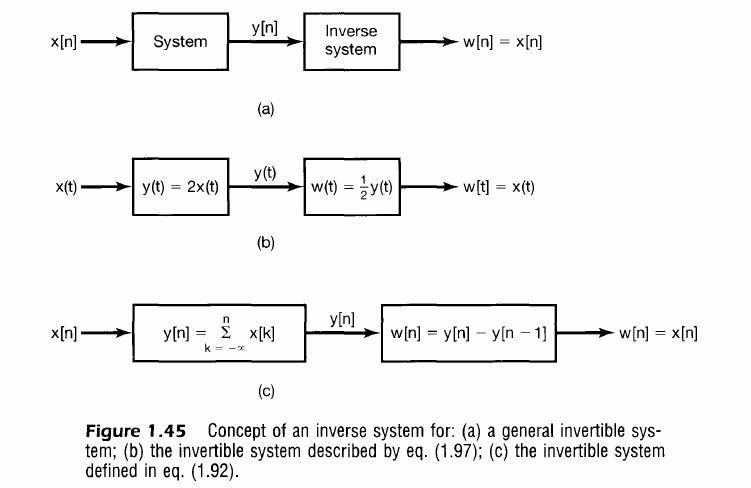
\includegraphics[width=10cm]{a13}
\end{center}
See that the series interconnection between the invertible system and its inverse system has an overall input-output relationship
same as that for the identity system.
As illustrated in the second graph, an example of an invertible
continuous-time system is 
\begin{equation*}
y(t)=2x(t)
\end{equation*}
for which the inverse system is
\begin{equation*}
w(t)=\frac{1}{2}y(t)
\end{equation*}
Another example is illustrated in the third block diagram, see that the accumulator is an invertible system:
\begin{equation*}
y[n]=\sum^n_{k=-\infty}x[k]
\end{equation*}
with inverse system
\begin{equation*}
w[n]=y[n]-y[n-1]
\end{equation*}
Examples of noninvertible systems include
\begin{equation*}
y[n]=0
\end{equation*}
or
\begin{equation*}
y(t)=x^2(t)
\end{equation*}
where a single output can correspond to different inputs.\\
(next page)\newpage
\noindent\textbf{Stability}\\
Another important system property is \textit{stability}. Informally, a stable system is one in which small inputs lead to
responses that do not diverge (grow uncontrollably).\\
\vspace{1mm}\\
More formally, if the input to a stable system is bounded (if its magnitude of the input does not grow without bound), then the
output must also be bounded and therefore cannot diverge. (this is the definition to take note of)\\
\vspace{1mm}\\
For instance consider the averaging system brought up earlier
\begin{equation*}
y[n]=\frac{1}{2M+1}\sum^{+M}_{k=-M}x[n-k]
\end{equation*}
Suppose that the input $x[n]$ is bounded in magnitude by some number, say $B$ for all values of $n$. Then the largest possible 
magnitude for $y[n]$ is also $B$ since it is the average. Therefore, $y[n]$ is bounded and the system is stable.\\
\vspace{1mm}\\
On the other hand, the accumulator sums all of the past values of the input, so the output will grow continually even if $x[n]$
is bounded---it is an unstable system.\\
\vspace{1mm}\\
A useful strategy to verify that a system is unstable is to look for a specific bounded input that leads to an unbounded
output. For instance consider 
\begin{equation*}
y(t)=tx(t)
\end{equation*}
See that a constant input $x(t)=1$ yields $y(t)=t$, which is unbounded. Since for any finite constant bound, $|y(t)|$ will exceed 
that bound at some $t$, this system is unstable.\\
\vspace{1mm}\\
Now consider a different system
\begin{equation*}
y(t)=e^{x(t)}
\end{equation*}
See that for an arbitrary positive number $B$, if $x(t)$ is bound by $B$, that is
\begin{equation*}
|x(t)|<B
\end{equation*}
or
\begin{equation*}
-B<x(t)<B
\end{equation*}
for all $t$, then $y(t)$ must satisfy
\begin{equation*}
e^{-B}<|y(t)|<e^B
\end{equation*}
Any input to this system bounded by an arbitrary positive number $B$ has a output guaranteed to be bounded by $e^B$---this system
is stable.
\newpage

\section{Basic system properties 2}
\textbf{Time invariance}\\
A system it \textit{time invariant} if a time shift in the input signal results in an identical time shift in the output
signal.\\
\vspace{1mm}\\
That is, if $y[n]$ is the output of a discrete-time, time-invariant system with input $x[n]$, then $y[n-n_0]$ is the output
when $x[n-n_0]$ is applied. In continuous time with $y(t)$ the output corresponding to the input $x(t)$, a time-invariant system
will have $y(t-t_0)$ as the output when $x(t-t_0)$ is the input.\\
\vspace{1mm}\\
\textbf{Examples}\\
Consider the continuous-time system
\begin{equation*}
y(t)=\sin[x(t)]
\end{equation*}
To check that this system is time invariant, we must determine whether the time-invariance property holds for \textit{any} input
and \textit{any} time shift $t_0$. Thus, letting $x_1(t)$ be an
arbitrary input to the system, with corresponding output
\begin{equation*}
y_1(t)=\sin[x_1(t)]
\end{equation*}
Now consider a second input $x_2$ obtained by shifting $x_1(t)$ in time
\begin{equation*}
x_2(t)=x_1(t-t_0)
\end{equation*}
The output corresponding to this input is
\begin{equation*}
y_2(t)=\sin[x_2(t)]=\sin[x_1(t-t_0)]
\end{equation*}
Now consider translating the output $y_1$, see that
\begin{equation*}
y_1(t-t_0)=\sin[x_1(t-t_0)]
\end{equation*}
Since $y_2$, the output of the shifted input, is the same as $y_1(t-t_0)$, which is if we had shifted the output instead, this
system is time invariant.\\
(next page)\newpage
\noindent\textbf{More examples}\\
As a second example, consider
\begin{equation*}
y[n]=nx[n]
\end{equation*}
See that time shifting the input doesn't correspond with an equivalent shift in the output---this is a time-varying system. 
This system represents one with a time-varying gain, even if we know the input value, we cannot determine the output value 
without knowing the current time.\\
\vspace{1mm}\\
For a counterexample, consider having input $x_1[n]=\delta[n]$, which yields an output $y_1[n]=0$ (since $n\delta[n]=0$). 
However, the input $x_2[n]=\delta[n-1]$ yields the output $y_2[n]=n\delta[n-1]=\delta[n-1]$---while $x_2[n]$ is a shifted 
version of $x_1[n]$, $y_2[n]$ is \textit{not} a shifted version of $y_1[n]$.\\
\vspace{1mm}\\
For a final example, consider the system
\begin{equation*}
y(t)=x(2t)
\end{equation*}
This system represents a time scaling. That is, $y(t)$ is a time-compressed (by a factor of 2) version of $x(t)$.
Intuitively then, any time shift in the input will also be compressed by a factor of 2, and it is for this reason that the system 
is not time invariant. Consider a counterexample: 
\begin{center}
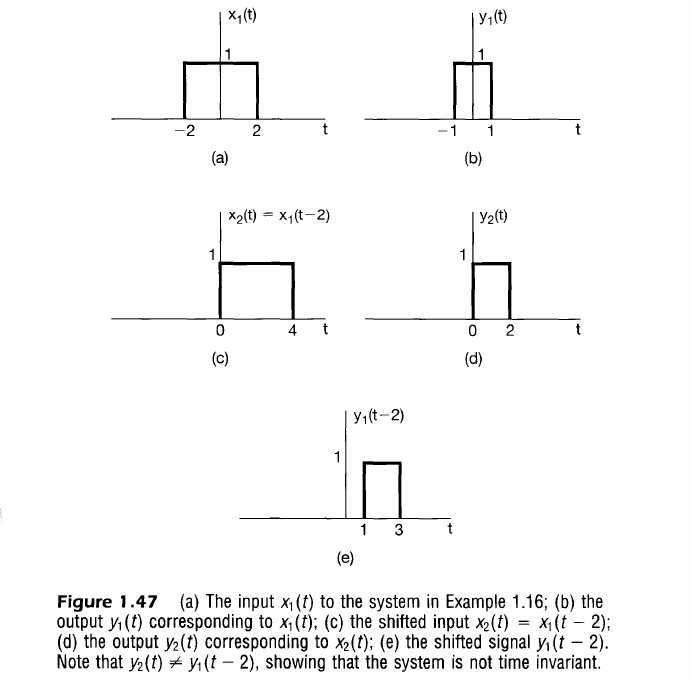
\includegraphics[width=8.5cm]{a14}
\end{center}
see that
if we shift the input signal by 2, the resulting output is not the same as if we had shifted the output signal by 2.\\
(next page)\newpage
\noindent\textbf{Linearity}\\
A \textit{linear system}, in continuous or discrete time, is a system that possesses the important property of superposition: If
an input consists of the weighted sum of several signals, then the output is the superposition---that is, the weighted sum---of
the responses of the system to each of those signals.\\
\vspace{1mm}\\
More precisely, letting $y_1(t)$ be the response of a continuous-time system to an input $x_1(t)$, 
and $y_2(t)$ the response to $x_2(t)$, the system is linear if:
\begin{enumerate}
\item The response to $x_1(t)+x_2(t)$ is $y_1(t)+y_2(t)$.
\item The response to $ax_1(t)$ is $ay(1)$, where $a$ is any complex constant.
\end{enumerate}
The first property is known as the \textit{additivity} propery, while the second the \textit{scaling} or \textit{homogeneity} 
property; the same definition holds for continuous time.
Note that a system can be linear without being time invariant, and it can be time invariant without being linear.\\
\vspace{1mm}\\
The two properties defining a linear system can be combined into a single statement:
\begin{align*}
\text{continuous time: }ax_1(t)+bx_2(t)&\to ay_1(t)+by_2(t)\\
\text{discrete time: }ax_1[n]+bx_2[n]&\to ay_1[n]+by_2[n]
\end{align*}
where $a$ and $b$ are any complex constants.\\
\vspace{1mm}\\
From this see that for a set of inputs $x_k[n],k=1,2,3,\ldots$ to a discrete-time linear system with corresponding outputs 
$y_k[n],k=1,2,3,\ldots$, then the response to a linear combination of these inputs given by 
\begin{equation*}
x[n]=\sum_ka_kx_k[n]=a_1x_1[n]+a_2x_2[n]+a_3x_3[n]+\ldots
\end{equation*}
is
\begin{equation*}
y[n]=\sum_ka_ky_k[n]=a_1y_1[n]+a_2y_2[n]+a_3y_3[n]+\ldots
\end{equation*}
This is known as the \textit{superposition property}, which holds for linear systems in both continuous and discrete time.\\
\vspace{1mm}\\
See that a direct consequence of the superposition property is that, for linear systems, an input which is zero for all time
results in an output which is zero for all time; if $x[n]\to y[n]$, then by the homogeneity property 
\begin{equation*}
0=0\cdot x[n]\to0\cdot y[n]=0
\end{equation*}
(next page)\newpage
\noindent\textbf{Examples}\\
Consider the system
\begin{equation*}
y(t)=tx(t)
\end{equation*}
To determine whether or not it is linear, we consider two arbitrary inputs $x_1(t)$ and $x_2(t)$.
\begin{align*}
x_1(t)&\to y_1(t)=tx_1(t)\\
x_2(t)&\to y_2(t)=tx_2(t)
\end{align*}
Now consider $x_3(t)$, a linear combination of $x_1(t)$ and $x_2(t)$:
\begin{equation*}
x_3(t)=ax_1(t)+bx_2(t)
\end{equation*}
where $a$ and $b$ are arbitrary scalars. See that for input $x_3(t)$, we have the output
\begin{align*}
y_3(t)&=tx_3(t)\\
&=t(ax_1(t)+bx_2(t))\\
&=atx_1(t)+btx_2(t)\\
&=ay_1(t)+by_2(t)
\end{align*}
So we conclude that the system is linear (also see that it is not time invariant).\\
\vspace{1mm}\\
For another example, consider the system
\begin{equation*}
y(t)=x^2(t)
\end{equation*}
as defining $x_1(t),x_2(t)$, and $x_3(t)$ as in the previous example, we have
\begin{align*}
x_1(t)\to y_1(t)=x^2_1(t)\\
x_2(t)\to y_2(t)=x^2_2(t)
\end{align*}
and 
\begin{align*}
x_3(t)\to y_3(t)&=x^2_3(t)\\
&=(ax_1(t)+bx_2(t))^2\\
&=a^2x^2_1(t)+b^2x^2_2(t)+2abx_1(t)x_2(t)\\
&=a^2y_1(t)+b^2y_2(t)+2abx_1(t)x_2(t)
\end{align*}
which isn't a superposition of the inputs, thus the system is not linear.\\
(next page)\newpage
\noindent\textbf{More examples}\\
It is important to remember that the scaling constants of the superposition criteria are allowed to be complex. Consider
the system
\begin{equation*}
y[n]=\text{Re}\{x[n]\}
\end{equation*}
This system is additive, but does not satisfy the homogeneity property, consider input
\begin{equation*}
x_1[n]=r[n]+is[n]
\end{equation*}
the corresponding output is 
\begin{equation*}
y_1[n]=r[n]
\end{equation*}
Now consider scaling $x_1[n]$ by a complex number, for instance $a=i$; defined as $x_2$:
\begin{align*}
x_2[n]&=ix_1[n]=i(r[n]+is[n])\\
&=-s[n]+ir[n]
\end{align*}
The corresponding output then is
\begin{equation*}
y_2[n]=\text{Re}\{x_2[n]\}=-s[n]
\end{equation*}
which is not equal to the scaled version of $y_1[n]$:
\begin{equation*}
ay_1[n]=ir[n]
\end{equation*}
thus the system violates the homogeneity property and is not linear.\\
(next page)\newpage
\noindent\textbf{Example---incrementally linear system}\\
Consider the system
\begin{equation*}
y[n]=2x[n]+3
\end{equation*}
This system is not linear, see that it violates the additivity property:
\begin{align*}
x_1[n]\to y_1[n]=2x_1[n]+3\\
x_2[n]\to y_2[n]=2x_2[n]+3
\end{align*}
where the response to $x_3[n]=x_1[n]+x_2[n]$ is
\begin{equation*}
y_3[n]=2(x_1[n]+x_2[n])+3
\end{equation*}
while 
\begin{equation*}
y_1[n]+y_2[n]=2(x_1[n]+x_2[n])+6
\end{equation*}
See that this system violates the property of linear systems where zero input yields zero output.\\
\vspace{1mm}\\
It may be surprising that the system here is nonlinear since it describes a linear equation. Intuitively, see that the output
of this system can be represented as the sum of the output of a linear system
\begin{equation*}
x[n]\to2x[n]
\end{equation*}
and another signal equal to the \textit{zero-input
response} of the system (when the input is zero), 
\begin{equation*}
y_0[n]=3
\end{equation*}
\begin{center}
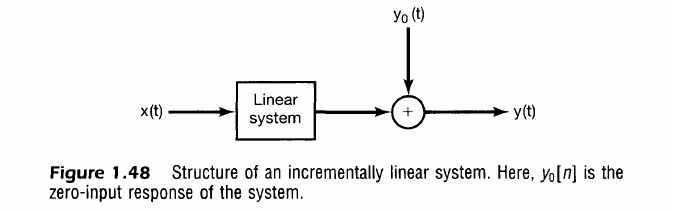
\includegraphics[width=10cm]{a15}
\end{center}
There are large classes of systems that can be represented like this, for which the overall system output
consists of the superposition of the response of a linear system with a zero-input response; these systems correspond to the class
of \textit{incrementally linear systems}.\\
\vspace{1mm}\\
The \textit{difference} between the resposnes to any two inputs to an incrementally system is a 
linear (additive and homogeneous) function of the \textit{difference} between the two inputs. For example, for inputs $x_1[n]$, 
$x_2[n]$ and corresponding outputs $y_1[n]$, $y_2[n]$ we have
\begin{equation*}
y_1[n]-y_2[n]=2x_1[n]+3-(2x_2[n]+3)=2[x_1[n]-x_2[n]]
\end{equation*}
\newpage

\chapter{Linear Time-Invariant Systems}
\section{Discrete-time convolution sum}
\textbf{Representing a discrete signal in terms of impulses}\\
The key idea in visualising how the discrete-time unit impulse can be used to construct any discrete-time signal is to think of a discrete-time signal as a sequence of individual impulses:
\begin{center}
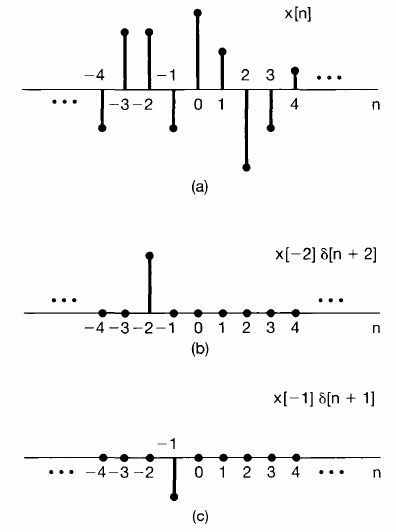
\includegraphics[width=3.5cm]{a16}
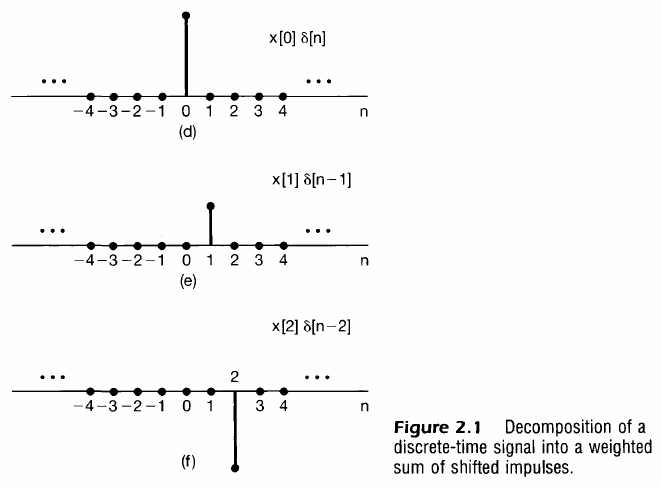
\includegraphics[width=6.5cm]{a17}\\
\end{center}
See that we can express express each value of $x[n]$ as an individual scaled, shifted impulse; for instance
\begin{align*}
x[-1]\delta[n+1]&=\begin{cases}x[-1],&n=-1\\
0,&n\neq-1\end{cases}\\
x[0]\delta[n]&=\begin{cases}x[0],&n=0\\
0,&n\neq0\end{cases}\\
x[1]\delta[n-1]&=\begin{cases}x[1],&n=1\\
0,&n\neq1\end{cases}
\end{align*}
More generally, see that we can write
\begin{align*}
x[n]=\ldots&+x[-3]\delta[n+3]+x[-2]\delta[n+2]+x[-1]\delta[n+1]
+x[0]\delta[n]\\
&+x[1]\delta[n-1]+x[2]\delta[n-2]+x[3]\delta[n-3]+\ldots
\end{align*}
For any value of $n$, only one of the terms on the right-hand side of the equation is nonzero, and the scaling associated
with that term is precisely $x[n]$. Writing this summation in a more compact form, we have
\begin{equation*}
x[n]=\sum^{+\infty}_{k=-\infty}x[k]\delta[n-k]
\end{equation*}
This equation is called the \textit{sifting property} of the discrete-time unit impulse; the summation `sifts' through
$x[k]$ and preserves only the value corresponding to $k=n$.\\
(next page)\newpage
\noindent\textbf{Convolution-sum representation of LTI systems}\\
The fact that $x[n]$ can be represented as a superposition of scaled versions of (time shifted) impulses, means that the response
of a linear system to $x[n]$ will be a \textit{superposition of the scaled responses of the system} to each of these shifted 
impulses.\\
\vspace{1mm}\\
Moreover, the property ot time invariance tells us that that the \textit{responses of a time-invariant system to the 
time-shifted unit 
impulses are simply time-shifted versions of one another}. The convolution-sum representation for discrete-time systems that 
are both linear and time invariant results from putting these two basic facts together.\\
\vspace{1mm}\\
\textbf{Linear, not necessarily time invariant response}\\
Consider the response of a linear (but possibly time-varying) system to an arbitrary input $x[n]$. We can represent
$x[n]$ as a linear combination of shifted impulses.\\
\vspace{1mm}\\
Letting $h_k[n]$ denote the response of the linear system to the shifted unit
impulse $\delta[n-k]$, see that the superposition property of linear systems means that the response $y[n]$ 
of a linear system to the input $x[n]$ is simply the weighted
linear combination of these basic responses:
\begin{equation*}
y[n]=\sum^{+\infty}_{k=-\infty}x[k]h_k[n]
\end{equation*}
The response value at a specific time $n$ of a linear system is the superposition of the `contributions' to that output point from each input (from all points in time).\\
(next page)\newpage
\noindent\textbf{Illustrated}\\
For instance, given the input signal $x[n]$ to a linear (non-time invariant) system with the responses $h_{-1}[n],h_{0}[n]$, and 
$h_{1}[n]$ to the signals $\delta[n+1],\delta[n]$, and $\delta[n-1]$:
\begin{center}
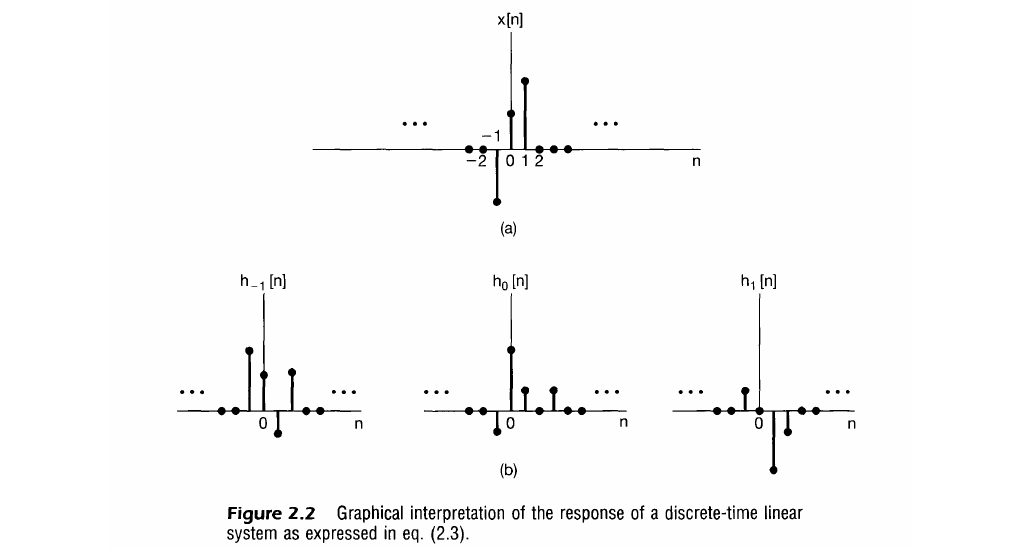
\includegraphics[width=10cm]{a18}
\end{center}
Since $x[n]$ can be written as a linear combination of the shifted impulses.
The system \textit{responses} to these time shifted impulses, $h$, scaled accordingly by their respective input value, sum to produce 
$y[n]$.
\begin{center}
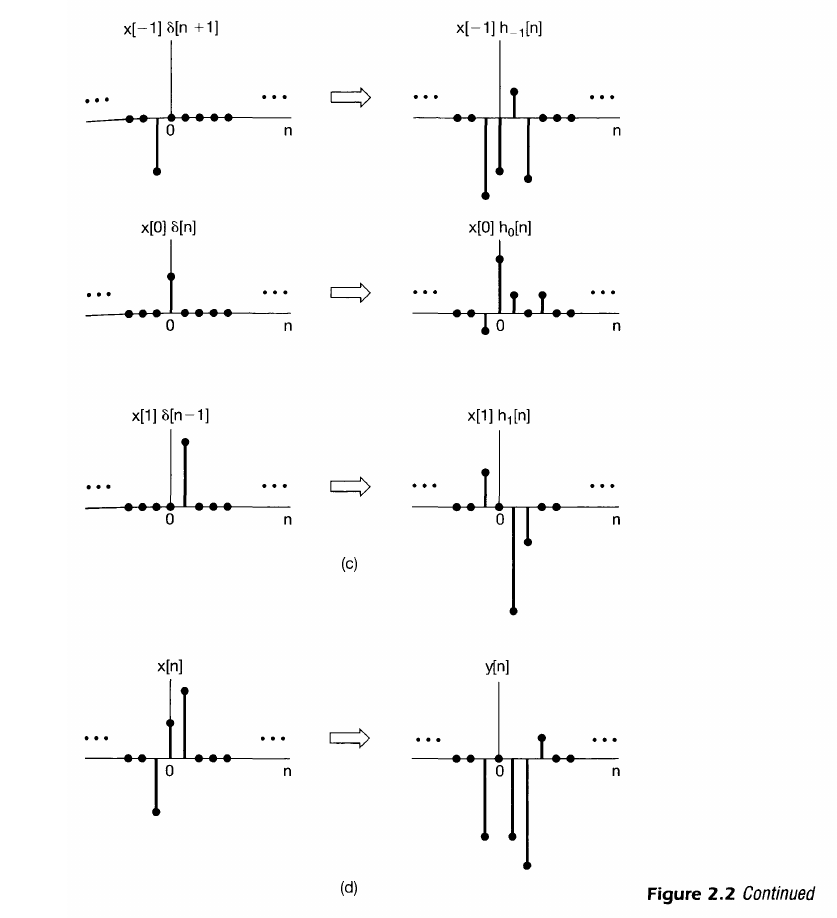
\includegraphics[width=7.8cm]{a19}
\end{center}
(This illustration only considers three points, but see that the summation on the previous page accounts for the possibility
that every input could contribute to a particular output point in time, thus the limits $-\infty$ to $\infty$)\\
(next page)\newpage
\noindent\textbf{LTI response---convolution sum}\\
In the previous case, the responses $h_k[n]$ need not be related to each other for different values of $k$. However,
if the linear system is also \textit{time invariant}, then these responses to time-shifted unit impulses are all 
\textit{time-shifted versions of each other}, meaning
\begin{equation*}
h_k[n]=h_0[n-k]
\end{equation*}
For notational convenience, we dr the subscript on $h_0[n]$ and define the \textit{unit impulse (sample) response} as 
\begin{equation*}
h[n]=h_0[n]
\end{equation*}
That is, when $h[n]$ is the output of the LTI system when $\delta[n]$ is the input, we have
\begin{equation*}
y[n]=\sum^{+\infty}_{k=-\infty}x[k]h[n-k]
\end{equation*}
This result is referred to as the \textit{convolution sum} or \textit{superposition sum}, and the operation on the right-hand
side is known as the \textit{convolution} of the sequences
$x[n]$ and $h[n]$, represented symbolically as
\begin{equation*}
y[n]=x[n]*h[n]
\end{equation*}
See that an LTI system is completely characterised by its response to a single signal, the unit impulse. As before, the actual
output is a superposition of the responses, but due to time invariance this time 
every response is just a time shift of each other.
\newpage

\section{Discrete-time convolution sum---examples}
These examples are crucial for a deeper understanding of the discrete convolution. For reference, the definition of the 
convolution sum: When $h[n]$ is the output of the LTI system when $\delta[n]$ is the input, we have output $y[n]$
\begin{equation*}
y[n]=\sum^{+\infty}_{k=-\infty}x[k]h[n-k]
\end{equation*}
\textbf{Example 1}\\
Consider an LTI system with impulse response $h[n]$ and input $x[n]$, as illustrated
\begin{center}
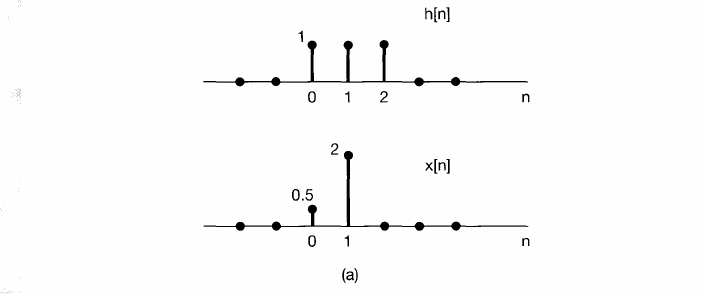
\includegraphics[width=10cm]{a20}
\end{center}
In this case, since only $x[0]$ and $x[1]$ are nonzero, the output (via convolution), simplifies to the expression
\begin{equation*}
y[n]=x[0]h[n-0]+x[1]h[n-1]=0.5h[n]+2h[n-1]
\end{equation*}
The sequences $0.5h[n]$ and $2h[n-1]$ are two `echoes' of the impulse response needed for the superposition involved in generating
$y[n]$, obtained by summing up each echo for each value of $n$.\\
(next page)\newpage
\textbf{Example 1 illustrated}
\begin{center}
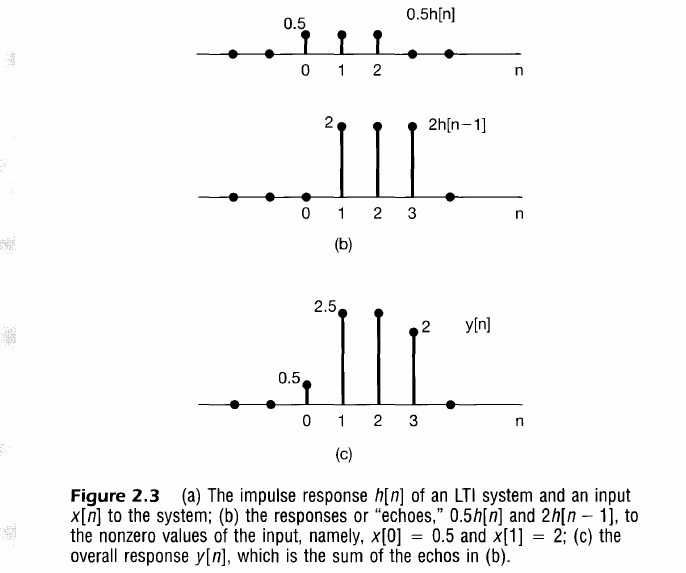
\includegraphics[width=10cm]{a21}\\
\end{center}
The output for point 0 depends on only on the first point of the impulse response at point 0, $x[0]h[0]$ 
(in this case there aren't any inputs before this point to produce other impulse responses to affect this). In contrast, the
output for point 1 depends on both the \textit{second} point of the impulse response at point 0, $x[0]h[1-0]$ and the 
\textit{first} point of the impulse response at point 1, $x[1]h[1-1]$. (see how this relates to the structure of the convolution sum)\\
\vspace{1mm}\\
\textbf{Alternative view of the convolution}\\
Consider the evaluation of the output value at a specific time $n$, a particularly convenient way of displaying this calculation
graphically begins with the two signals $x[k]$ and
$h[n-k]$ viewed as functions of $k$.\\
\vspace{1mm}\\
Multiplying these two functions, we obtain a sequence $g[k]=x[k]h[n-k]$, which, at each time $k$, can be seen as representing
the contribution of $x[k]$ to the output at time $n$. 
Summing all the samples in the sequence of $g[k]$ yields the output value at the selected time $n$.\\
\vspace{1mm}\\
Thus, to calculate $y[n]$ for all values of $n$ requires repeating this procedure for each value of $n$. Fortunately, changing
the value of $n$ has a very simple graphical interpretation for
the two signals $x[k]$ and $h[n-k]$, viewed as functions of $k$.
The following examples illustrate this.\\
(next page)\newpage
\noindent\textbf{Example 2---view as a function of $k$}\\
Let us consider again the convolution problem encountered in the previous example. Now we have the sequences $x[k]$ and 
$h[n-k]$, for $n$ fixed and viewed as a function of $k$; see that
the graph of $h[n-k]$ is a time reversal and shift---to the \textit{right} if $n$ is positive and \textit{left} if $n$ 
is negative:
\begin{center}
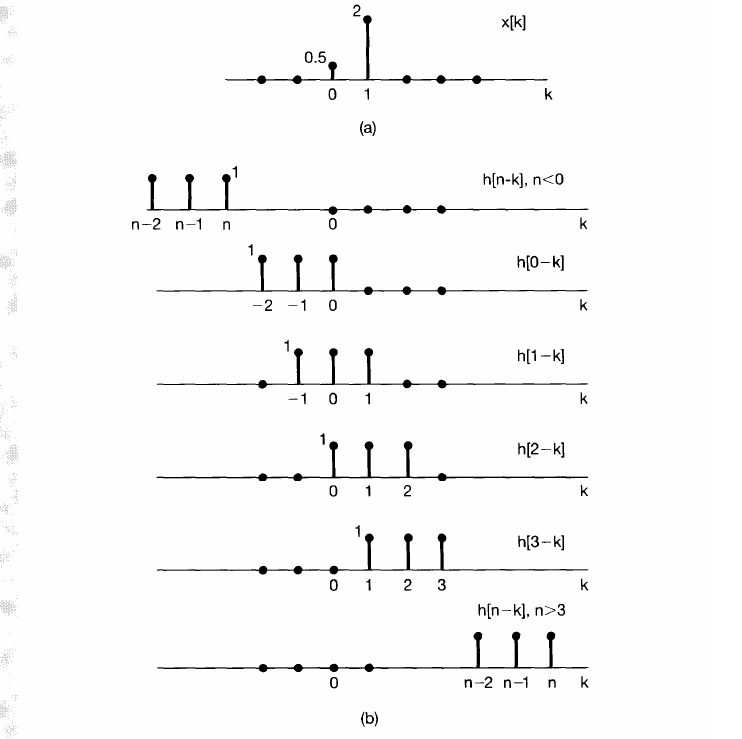
\includegraphics[width=9cm]{a22}\\
\end{center}
Having sketched $x[k]$ and $h[n-k]$ for a given $n$, we multiply the two signal and sum over all values of $k$ 
(like a dot product) to get $y[n]$. (We multiply and sum up the points where the graphs `overlap')\\
\vspace{1mm}\\
(Intuit that the view in the first example is the same as `reversing' the impulse response and moving it along the input like a 
sliding window, which is essentially what is happening here.)\\
\vspace{1mm}\\
For $n<0$, neither of the graphs overlap at points where both are nonzero, so $y[n]=0$ for $n<0$. For $n=0$, since the product
of the sequence $x[k]$ and the sequence $h[0-k]$ has only one nonzero sample (at $k=0$), we have
\begin{equation*}
y[0]=\sum^\infty_{k=-\infty}x[k]h[0-k]=x[0]h[0]=0.5
\end{equation*}
(next page)\newpage
\noindent\textbf{cont. from example 2}\\
The other examples have more `overlapping' points:
\begin{align*}
y[1]&=\sum^\infty_{k=-\infty}x[k]h[1-k]=0.5+2.0=2.5\\
y[2]&=\sum^\infty_{k=-\infty}x[k]h[2-k]=0.5+2.0=2.5\\
y[3]&=\sum^\infty_{k=-\infty}x[k]h[3-k]=2.0
\end{align*}
(next page)\newpage
\noindent\textbf{Example 3}\\
Consider input $x[n]$ and unit impulse $h[n]$ given by
\begin{align*}
x[n]&=\alpha^nu[n]\\
h[n]&=u[n]
\end{align*}
where $0<a<1$:
\begin{center}
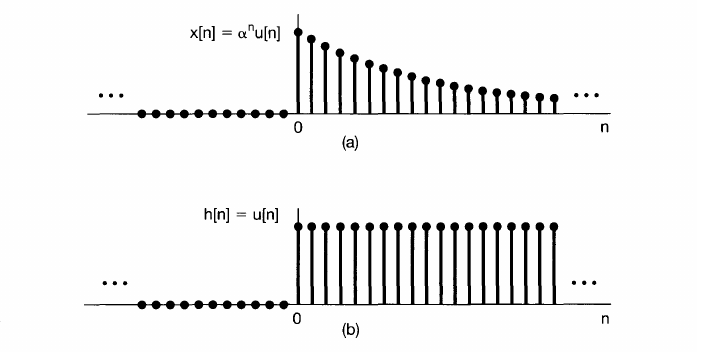
\includegraphics[width=9cm]{a23}\\
\end{center}
As before, consider $x[k]$ and $h[n-k]$ for different $n$:
\begin{center}
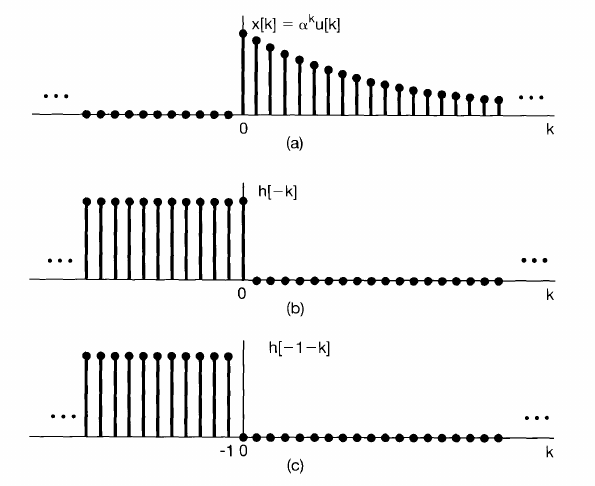
\includegraphics[width=5cm]{a24}
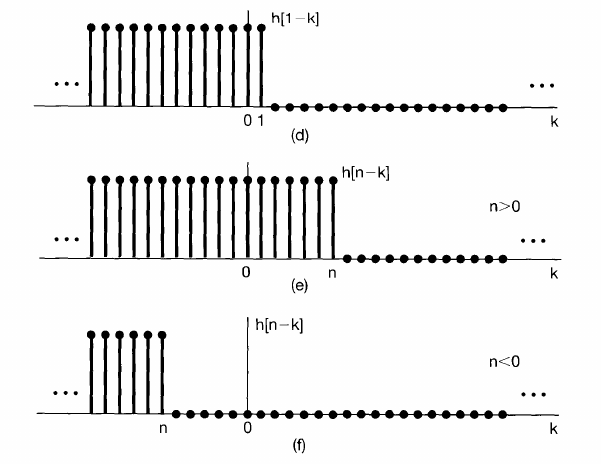
\includegraphics[width=5cm]{a25}
\end{center}
For $n<0$ there is no overlap between nonzero points in $x[k]$ and $h[n-k]$, so $y[n]=0$ for $n<0$. See that for $n\geq0$,
\begin{equation*}
x[k]h[n-k]=\begin{cases}
\alpha^k,&0\leq k\leq n\\
0,&\text{otherwise}
\end{cases}
\end{equation*}
Thus for $n\geq0$, the usual infinite limits are superfluous, and we can write 
\begin{equation*}
y[n]=\sum^n_{k=0}\alpha^k
\end{equation*}
this is a geometric series, we can write
\begin{equation*}
y[n]=\sum^n_{k=0}\alpha^k=\frac{1-\alpha^{n+1}}{1-\alpha}\quad
\text{for }n\geq0
\end{equation*}
(see appendix for sum of geometric series formula)\\
(next page)\newpage
\noindent\textbf{cont. example 3}\\
We had
\begin{equation*}
y[n]=\sum^n_{k=0}\alpha^k=\frac{1-\alpha^{n+1}}{1-\alpha}\quad
\text{for }n\geq0
\end{equation*}
which can be rewritten as
\begin{equation*}
y[n]=\left(\frac{1-\alpha^{n+1}}{1-\alpha}\right)u[n]
\end{equation*}
Illustrated:
\begin{center}
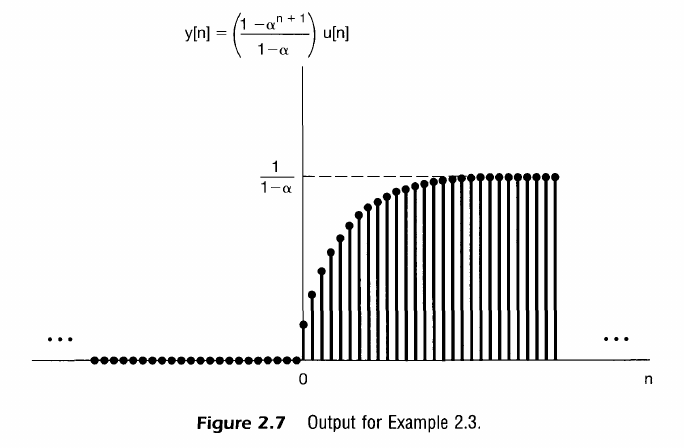
\includegraphics[width=10cm]{a26}\\
\end{center}
See that the convolution operation can be described as a `sliding' of the sequence $h[n-k]$ past $x[k]$ 
(as we increase $n$ the $h[n-k]$ graph just gets shifted to the right).\\
\vspace{1mm}\\
For example, suppose we have evaluated $y[n]$ for some particular value of $n$, say $n=n_0$, meaning we have sketched $h[n_0-k]$, 
multiplied it by $x[k]$, and summed the results over all $k$.
To evaluate $y[n]$ at the next value of $n$, so $n=n_0+1$, we sketch $h[(n_0+1)-k]$; 
however, we can do this by simply translating $h[n_0-k]$ to the right by one point.\\
\vspace{1mm}\\
Repeating this for each successive $n$ demonstrates this `sliding' idea.\\
(next page)\newpage
\noindent\textbf{Example 4}\\
Consider an LTI system with input $x[n]$ and unit impulse response $h[n]$ specified as
\begin{align*}
x[n]&=2^nu[-n]\\
h[n]&=u[n]
\end{align*}
\begin{center}
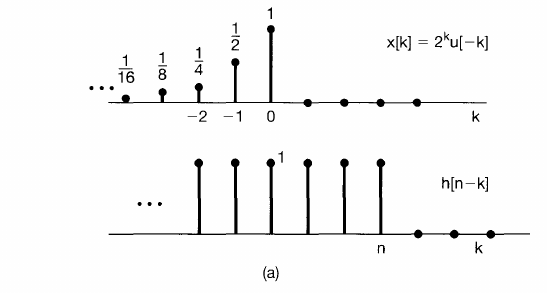
\includegraphics[width=10cm]{a27}\\
\end{center}
See that $x[k]$ is zero for $k>0$ and $h[n-k]$ is zero for $k>n$.
Also see that regardless of $n$, the sequence $x[k]h[n-k]$ always has nonzero samples along the $k$-axis, and when $n\geq0$, 
$x[k]h[n-k]$ has nonzero samples in the interval $k\leq0$. As such we can write, for $n\geq0$
\begin{equation*}
y[n]=\sum^0_{k=-\infty} x[k]h[n-k]=\sum^0_{k=-\infty}2^k
\end{equation*}
and for $n<0$, $x[k]h[n-k]$ has nonzero samples for $k\leq n$. It follows that, for $n<0$
\begin{equation*}
y[n]=\sum^n_{k=-\infty} x[k]h[n-k]=\sum^n_{k=-\infty}2^k
\end{equation*}
(next page)\newpage
\noindent\textbf{cont. example 4}\\
In both cases we can simplify using the the formula for summing geometric series (see appendix)
\begin{equation*}
\sum^\infty_{k=0}\alpha^k=\frac{1}{1-\alpha}
\end{equation*}
Where for the $n\geq0$ case, by performing a change of variable 
$r=-k$,
\begin{equation*}
y[n]=\sum^0_{k=-\infty}2^k=\sum^{\infty}_{r=0}\left(\frac{1}{2}\right)^r=\frac{1}{1-(1/2)}=2
\end{equation*}
For the $n<0$ case, by performing a change of variable $l=-k$, and then $m=l+n$,
\begin{align*}
y[n]=\sum^n_{k=-\infty}2^k&=\sum^{\infty}_{l=-n}\left(\frac{1}{2}\right)^l=\sum^{\infty}_{m=0}\left(\frac{1}{2}\right)^{m-n}
\\
&=\left(\frac{1}{2}\right)^{-n}\sum^{\infty}_{m=0}\left(\frac{1}{2}\right)^{m}=2^n\cdot2=2^{n+1}
\end{align*}
\begin{center}
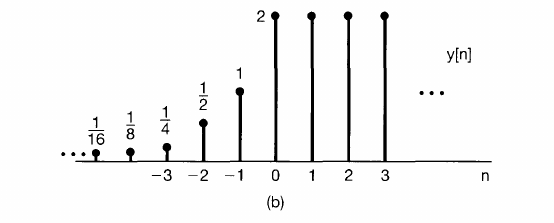
\includegraphics[width=10cm]{a28}\\
\end{center}
\newpage

\section{Continuous-time---the convolution integral}
\textbf{Representating a continuous signal in terms of impulses}\\
We develop a continuous-time conterpart of the discrete-time `sifting' property. Consider a riemann-sum like approximation, $\hat{x}(t)$, to a continuous-time signal $x(t)$:
\begin{center}
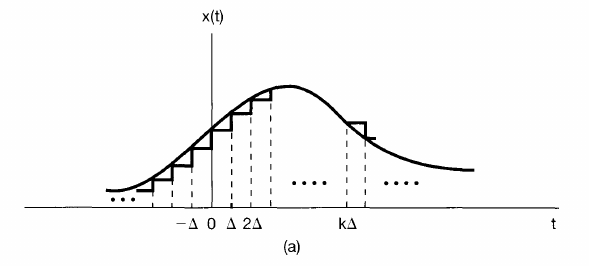
\includegraphics[width=10cm]{a29}\\
\end{center}
This approximation can be expressed as a linear combination of delayed rectangular pulses. If we define
\begin{equation*}
\delta_\Delta(t)=\begin{cases}
\frac{1}{\Delta},&0\leq t<\Delta\\
0,&\text{otherwise}
\end{cases}
\end{equation*}
then since $\Delta\delta_\Delta(t)$ has unit amplitude, we have the expression
\begin{equation*}
\hat{x}(t)=\sum^{+\infty}_{k=-\infty}x(k\Delta)\delta_\Delta(t-k\Delta)\Delta
\end{equation*}
($\delta_\Delta$ `turns on' a specific rectangle, $x$ specifies its height, and $\Delta$ the base length) See that for any $t$,
only one term in the summation on the right is nonzero.\\
\vspace{1mm}\\
As we let $\Delta$ approach 0, the approximation $\hat{x}(t)$ becomes better, and in the limit equals $x(t)$, therefore we write
\begin{equation*}
x(t)=\lim_{\Delta\to0}\sum^{+\infty}_{k=-\infty}x(k\Delta)\delta_\Delta(t-k\Delta)\Delta
\end{equation*}
Also, as $\Delta\to0$, the summation approaches an integral; see that since the limit of $\delta\to0$ of $\delta_\Delta(t)$ is
the unit impulse function $\delta(t)$, we have
\begin{equation*}
x(t)=\int^{+\infty}_{-\infty}x(\tau)\delta(t-\tau)d\tau
\end{equation*}
This should be viewed as an idealisation in the sense that, for any $\Delta$ `small enough', the approximation by this summation
is essentially exact for any practical purpose. The
integral then represents an idealisation of the summation by
taking $\Delta$ to be vanishingly small.\\
(next page)\newpage
\noindent\textbf{Viewed as a function of $\tau$}\\
See that when the signal $\delta(t-\tau)$ is viewed as a function of $\tau$ with $t$ fixed, it is still a unit impulse located at 
$\tau=t$:
\begin{center}
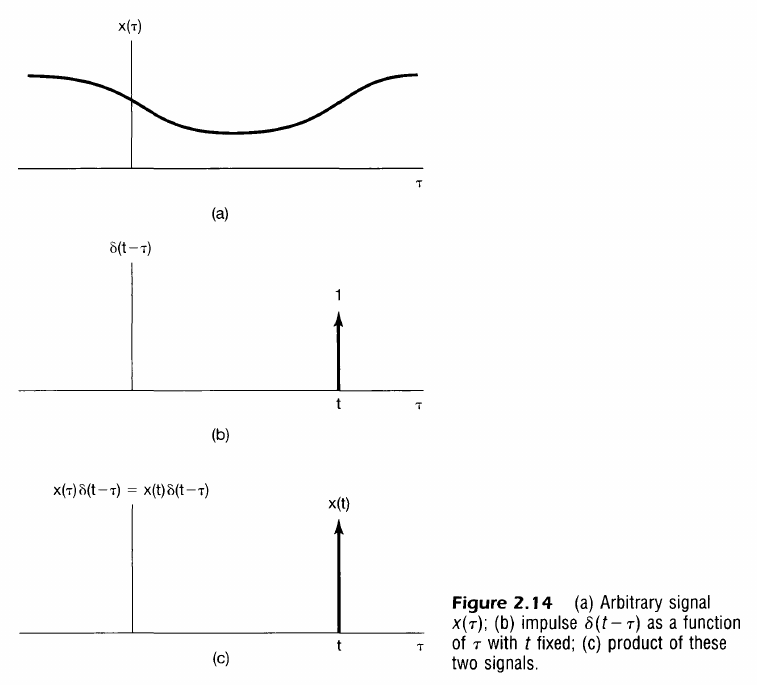
\includegraphics[width=10cm]{a30}\\
\end{center}
As such, we have
\begin{equation*}
x(\tau)\delta(t-\tau)=x(t)\delta(t-\tau)
\end{equation*}
which is just a scaled impulse at $\tau=t$ with area equal to $x(t)$. See that this can be used to show the statement on the
previous page
\begin{equation*}
\int^{+\infty}_{-\infty}x(\tau)\delta(t-\tau)d\tau=
\int^{+\infty}_{-\infty}x(t)\delta(t-\tau)d\tau=
x(t)\int^{+\infty}_{-\infty}\delta(t-\tau)d\tau=x(t)
\end{equation*}
Emphasising the interpretation of the $x(t)$ being represented as a sum (or more precisely, an integral) of weighted, shifted
impulses.\\
(next page)\newpage
\noindent\textbf{Continuous-time impulse response}\\
We could represent $\hat{x}(t)$ as a sum of scaled and shifted versions of the basic pulse signal $\delta_\Delta(t)$.
\begin{equation*}
\hat{x}(t)=\sum^{+\infty}_{k=-\infty}x(k\Delta)\delta_\Delta(t-k\Delta)\Delta
\end{equation*}
Consequently, the response $\hat{y}(t)$ of a linear system to this signal will be the superposition of the responses to the scaled
and shifted versions of $\delta_\Delta(t)$.\\
\vspace{1mm}\\
Specifically, let us define $\hat{h}_{k\Delta}(t)$ as the response of an LTI system to the input $\delta_\Delta(t-k\Delta)$, then 
by superposition we have
\begin{equation*}
\hat{y}(t)=\sum^{+\infty}_{k=-\infty}x(k\Delta)\hat{h}_{k\Delta}(t)\Delta
\end{equation*}
Now consider what happens as $\Delta$ becomes vanishingly small, meaning $\Delta\to0$. $\hat{x}(t)$ becomes an increasingly good 
approximation to $x(t)$, and in fact, the two coincide as $\Delta\to0$.\\
\vspace{1mm}\\
Consequently, the response to $\hat{x}(t)$, namely, $\hat{y}(t)$, must converge to $y(t)$, the response to the actual input 
$x(t)$. Either way, we say that for $\Delta$ `small enough', the duration of the pulse $\delta_\Delta(t-k\Delta)$ is of no 
significance, in that, as far as the system is concerned, the 
response to this pulse is essentially the same as the response to a unit impulse as $\Delta\to0$:
\begin{center}
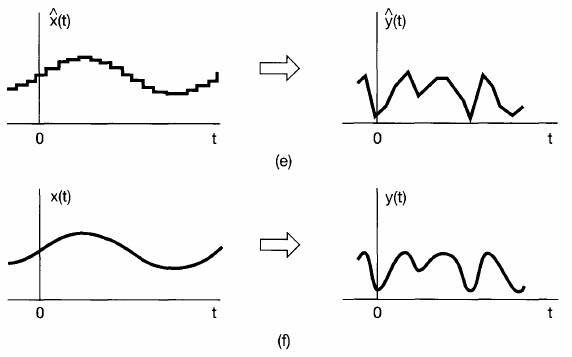
\includegraphics[width=9cm]{a31}\\
\end{center}
Since the pulse $\delta_\Delta(t-k\Delta)$ corresponds to a shifted unit impulse as $\Delta\to0$, the response 
$\hat{h}_{k\Delta}(t)$ to this input also becomes the impulse response in the limit. As such we have
\begin{equation*}
y(t)=\lim_{\Delta\to0}\sum^{+\infty}_{k=-\infty}x(k\Delta)
\hat{h}_{k\Delta}(t)\Delta
\end{equation*}
(next page)\newpage
\noindent\textbf{cont.}\\
We had
\begin{equation*}
y(t)=\lim_{\Delta\to0}\sum^{+\infty}_{k=-\infty}x(k\Delta)
\hat{h}_{k\Delta}(t)\Delta
\end{equation*}
As $\Delta\to0$, the summation on the right-hand side becomes an integral:
\begin{equation*}
y(t)=\int^{+\infty}_{-\infty}x(\tau)h_\tau(t)d\tau
\end{equation*}
This interpretation is analagous to the one earlier, where any input $x(t)$ can be represented as 
\begin{equation*}
x(t)=\int^{+\infty}_{-\infty}x(\tau)\delta(t-\tau)d\tau
\end{equation*}
$x(t)$ is essentially represented as a `sum', which, by linearity, leads to $y(t)$ being represented as a superposition of 
responses to each impulse in the `sum'.\\
\vspace{1mm}\\
\textbf{Convolution integral}\\
$y(t)$ as decribed above represents the general form of the response of a linear system in continuous time. 
If, in addition to being linear, the system is also time invariant, then the response to the impulse $\delta(t-\tau)$ is 
just the response to $\delta(t)$ shifted by $\tau$ from the origin, meaning $h_\tau(t)=h_0(t-\tau)$.\\
\vspace{1mm}\\
For notational convenience,
we can then drop the subscript and define the unit impulse response $h(t)$ (the response to $\delta(t)$) as
\begin{equation*}
h(t)=h_0(t)
\end{equation*}
In this case, the expression for the $y(t)$ above becomes
\begin{equation*}
y(t)=\int^{+\infty}_{-\infty}x(\tau)h(t-\tau)d\tau
\end{equation*}
This is referred to as the \textit{convolution integral} or the \textit{superposition integral}, the continuous-time counterpart
of the convolution sum, representing a continuous-time LTI system in terms of its response to a unit impulse, written symbolically
as
\begin{equation*}
y(t)=x(t)*h(t)
\end{equation*}
See that a continuous-time LTI system is completely characterised by its impulse response---a single elementary signal.\\
\vspace{1mm}\\
\textbf{Evaluation by visualisation in terms of $\tau$}\\
The procedure for evaluating the convolution integral is similar to the discrete-time counterpart: we first obtain the signal
$h(t-\tau)$ regarded as a function of $\tau$ with $t$ fixed; this is a reflection about the origin, shifted to the right by 
$t$ if $t>0$ or left if $t<0$. Next multiply $x(\tau)$ and $h(t-\tau)$ and integrate the product over infinity. (see examples)
\newpage

\section{Convolution integral---examples}
\textbf{Example 1}\\
Consider letting $x(t)$ be the input to an LTI system with unit impulse response $h(t)$, where
\begin{equation*}
x(t)=e^{-at}u(t),\quad a>0
\end{equation*}
and 
\begin{equation*}
h(t)=u(t)
\end{equation*}
\begin{center}
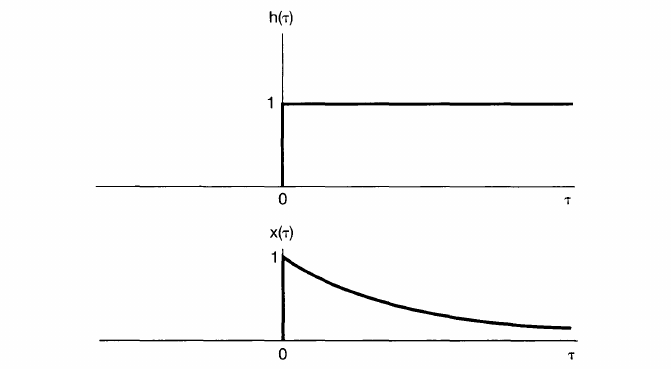
\includegraphics[width=9cm]{a32}\\
\end{center}
See that plotting $h(t-\tau)$ with $\tau$ as the horizontal axis:
\begin{center}
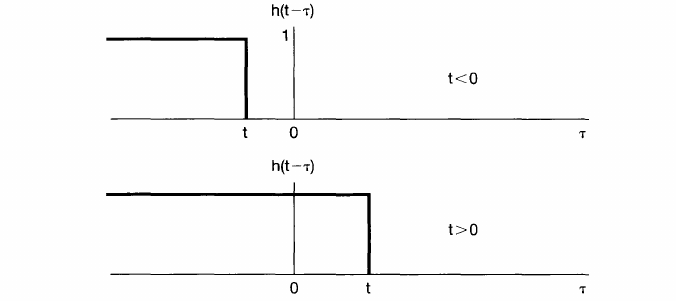
\includegraphics[width=9cm]{a33}\\
\end{center}
See that for $t<0$, the product of $x(\tau)$ and $h(t-\tau)$ is zero, and consequently, $y(t)$ is zero. While for
$t>0$,
\begin{equation*}
x(\tau)h(t-\tau)=\begin{cases}
e^{-a\tau},&0<\tau<t\\
0,&\text{otherwise}
\end{cases}
\end{equation*}
As such, the convolution integral to compute $y(t)$ for $t>0$ looks like
\begin{align*}
y(t)=\int^t_0e^{-a\tau}d\tau&=
\left.-\frac{1}{a}e^{-a\tau}\right|^t_0\\
&=\frac{1}{a}(1-e^{-at})
\end{align*}
(next page)\newpage
\noindent\textbf{cont. example 1}\\
We had $y(t)=0$ for $t<0$, and for $t>0$ we had
\begin{equation*}
y(t)=\frac{1}{a}(1-e^{-at})
\end{equation*}
for all $t$, we can write
\begin{equation*}
y(t)=\frac{1}{a}(1-e^{-at})u(t)
\end{equation*}
\begin{center}
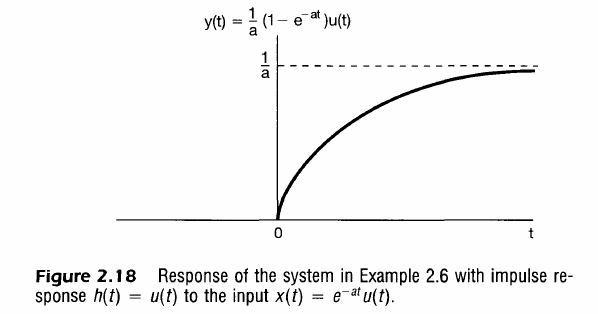
\includegraphics[width=9cm]{a34}\\
\end{center}
(next page)\newpage
\noindent\textbf{Example 2}\\
Consider the convolution of the following two signals
\begin{align*}
x(t)&=\begin{cases}1,&0<t<T\\
0,&\text{otherwise}\end{cases}\\
h(t)&=\begin{cases}t,&0<t<2T\\
0,&\text{otherwise}\end{cases}
\end{align*}
Now consider the graphs of $x(\tau)$ and $h(t-\tau)$ plotted for different values of $t$:
\begin{center}
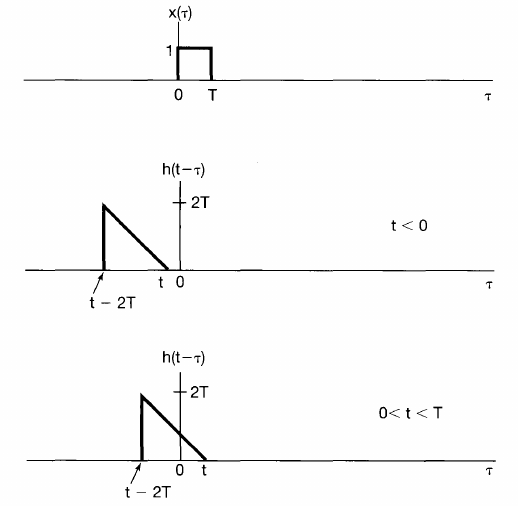
\includegraphics[width=5cm]{a35}
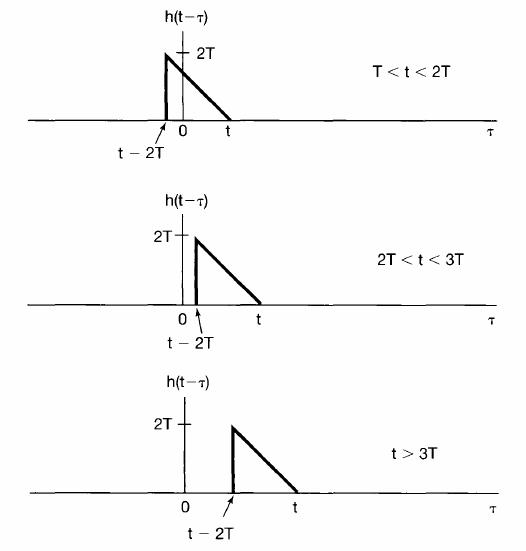
\includegraphics[width=5cm]{a36}
\end{center}
See that the convolution integral is different depending on the value of $t$:
\begin{equation*}
y(t)=\begin{cases}
0,&t<0\\
\int^t_0-\tau+t\,d\tau,&0<t<T\\
\int^T_0-\tau+t\,d\tau,&T<t<2T\\
\int^T_{t-2T}-\tau+t\,d\tau,&2T<t<3T\\
0,&3T<t
\end{cases}
\end{equation*}
\begin{center}
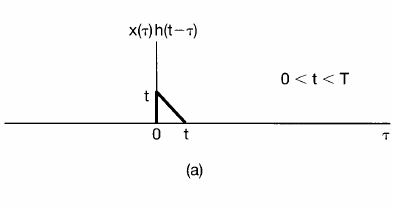
\includegraphics[width=5cm]{a37}
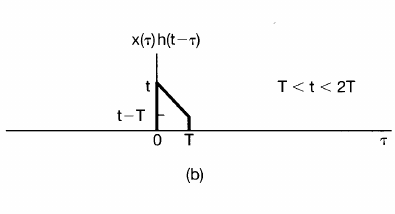
\includegraphics[width=5cm]{a38}\\
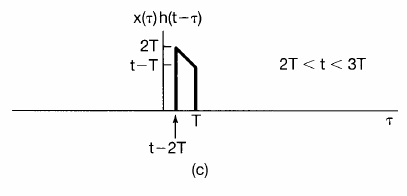
\includegraphics[width=6cm]{a39}\\
\end{center}
(next page)\newpage
\noindent\textbf{cont. example 2}\\
Each convolution integral evaluates to
\begin{equation*}
y(t)=\begin{cases}
0,&t<0\\
\frac{1}{2}t^2,&0<t<T\\
Tt-\frac{1}{2}T^2,&T<t<2T\\
-\frac{1}{2}t^2+Tt+\frac{3}{2}T^2,&2T<t<3T\\
0,&3T<t
\end{cases}
\end{equation*}
\begin{center}
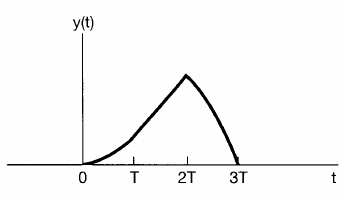
\includegraphics[width=9cm]{a40}
\end{center}
(next page)\newpage
\noindent\textbf{Example 3}\\
Consider the convolution between the two signals
\begin{align*}
x(t)&=e^{2t}u(-t)\\
h(t)&=u(t-3)
\end{align*}
\begin{center}
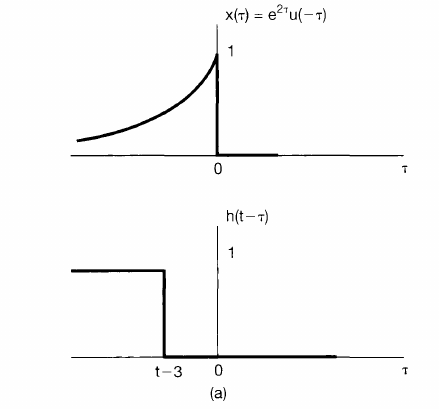
\includegraphics[width=7cm]{a41}
\end{center}
Observe that $x(\tau)$ and $h(t-\tau)$ have regions of nonzero overlap regardless of the value of $t$. 
When $t-3\leq0$, the product of $x(\tau)$ and $h(t-\tau)$ is nonzero for $-\infty<\tau<t-3$; the convolution integral becomes
\begin{equation*}
y(t)=\int^{t-3}_{-\infty}e^{2\tau}d\tau=\frac{1}{2}e^{2(t-3)}
\end{equation*}
For $t-3\geq0$, the product $x(\tau)h(t-\tau)$ is only nonzero for $-\infty<\tau<0$, so the convolution integral is
\begin{equation*}
y(t)=\int^0_{-\infty}e^{2\tau}d\tau=\frac{1}{2}
\end{equation*}
\begin{center}
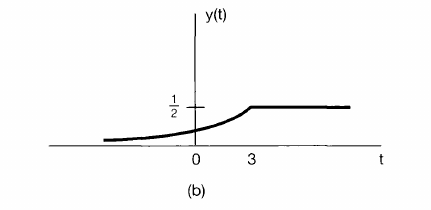
\includegraphics[width=9cm]{a42}
\end{center}
\newpage

\section{Properties of LTI systems 1}
For reference, we can represent continuous and discrete-time LTI systems in terms of their unit impulse responses; in
discrete-time this takes the form of the convolution sum, while its continuous-time counterpart is the convolution integral:
\begin{align*}
y[n]&=\sum^{+\infty}_{k=-\infty}x[k]h[n-k]=x[n]*h[n]\\
y(t)&=\int^{+\infty}_{-\infty}x(\tau)h(t-\tau)d\tau=x(t)*h(t)
\end{align*}
It is important to emphasise that this property holds in general \textit{only} for LTI systems (since the entire derivation
is based on this).\\
\vspace{1mm}\\
\textbf{Commutativity}\\
Convolution in both continuous and discrete time is \textit{commutative}. That is, in discrete time
\begin{equation*}
x[n]*h[n]=h[n]*x[n]=\sum^{+\infty}_{k=-\infty}h[k]x[n-k]
\end{equation*}
and in continuous time
\begin{equation*}
x(t)*h(t)=h(t)*x(t)=\int^{+\infty}_{-\infty}h(\tau)x(t-\tau)d\tau
\end{equation*}
These expressions can verified by means of a substitution of variables. In the discrete-time case, 
substituting $r=n-k$:
\begin{align*}
x[n]*h[n]&=\sum^{+\infty}_{k=-\infty}x[k]h[n-k]=
\sum^{-\infty}_{r=\infty}x[n-r]h[r]\\
&=\sum^{\infty}_{r=-\infty}x[n-r]h[r]=h[n]*x[n]
\end{align*}
and in the continuous case, substituting $r=t-\tau$:
\begin{align*}
x(t)*h(t)&=\int^{+\infty}_{-\infty}x(\tau)h(t-\tau)d\tau
=\int_{+\infty}^{-\infty}-x(t-r)h(r)dr\\
&=\int^{+\infty}_{-\infty}x(t-r)h(r)dr=h(t)*x(t)
\end{align*}
In the context of computing the convolution, this means that the step where a signal is reflected and shifted according to $n$ 
or $t$ can be done with either $x$ or $h$ in both discrete and continuous time.
One form may be easier to visualise, but both forms always result in the same answer.\\
(next page)\newpage
\noindent\textbf{Distributivity}\\
Convolution is also \textit{distributive}. Specifically, convolution distributes over addition, meaning in discrete time
\begin{equation*}
x[n]*(h_1[n]+h_2[n])=x[n]*h_1[n]+x[n]*h_2[n]
\end{equation*}
and in continuous time
\begin{equation*}
x(t)*[h_1(t)+h_2(t)]=x(t)*h_1(t)+x(t)*h_2(t)
\end{equation*}
This can be verified by direct subsitution into the convolution sum/integral.\\
\vspace{1mm}\\
See this means that the system
\begin{equation*}
y(t)=x(t)*h_1(t)+x(t)*h_2(t)
\end{equation*}
and the system
\begin{equation*}
y(t)=x(t)*[h_1(t)+h_2(t)]
\end{equation*}
are identical. There is an analagous interpretation in discrete time.\\
\vspace{1mm}\\
Illustrated using block diagrams, the two are identical:
\begin{center}
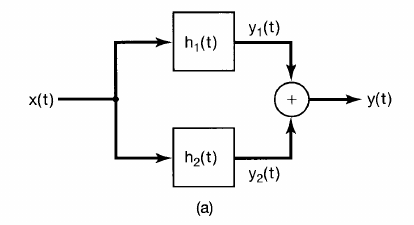
\includegraphics[width=5cm]{a43}
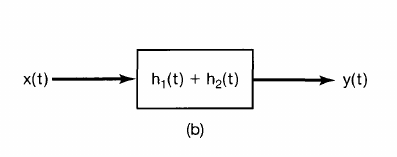
\includegraphics[width=5cm]{a44}
\end{center}
See also that as a consequence of bothe the commutative and distributive properties, we have
\begin{equation*}
[x_1[n]+x_2[n]]*h[n]=x_1[n]*h[n]+x_2[n]*h[n]
\end{equation*}
and
\begin{equation*}
[x_1(t)+x_2(t)]*h(t)=x_1(t)*h(t)+x_2(t)*h(t)
\end{equation*}
this means that the response of an LTI system to the sum of two inputs must equal the sum of the responses to each input 
individually.\\
(next page)\newpage
\noindent\textbf{Associativity}\\
Convolution is \textit{associative}; that is, in discrete time
\begin{equation*}
x[n]*(h_1[n]*h_2[n])=(x[n]*h_1[n])*h_2[n]
\end{equation*}
and in continuous time
\begin{equation*}
x(t)*[h_1(t)*h_2(t)]=[x(t)*h_1(t)]*h_2(t)
\end{equation*}
This property can be proven by straigntforward manipulation of the summations and integrals. In discrete time (the infinite limit
case obscures understanding, so assuming the convolution product is nonzero only for $0<k<n$ (or $t$)),
\begin{align*}
((f*g)*h)[n]&=\sum^{n}_{k=0}(f*g)[k]h[n-k]\\
&=\sum^{n}_{k=0}\left(\sum^k_{l=0}f[l]g[k-l]\right)h[n-k]\\
&=\sum_{0\leq l\leq k\leq n}f[l]g[k-l]h[n-k]\\
&=\sum^n_{l=0}\sum^n_{k=l}f[l]g[k-l]h[n-k]\\
&=\sum^n_{l=0}f[l]\left(\sum^{n-l}_{r=0}g[r]h[n-r-l]\right)\\
&=\sum^n_{l=0}f[l](g*h)[n-l]\\
&=(f*(g*h))[n]
\end{align*}
In the third last step we subsitute $r=k-l$. The continuous case is analagously:
\begin{align*}
((f*g)*h)(t)&=\int^t_{0}(f*g)(\tau)h(t-\tau)d\tau\\
&=\int^t_{\tau=0}\left(\int^\tau_{s=0}f(s)g(\tau-s)ds\right)h(t-\tau)d\tau\\
&=\iint_{0\leq s\leq\tau\leq t}f(s)g(\tau-s)h(t-\tau)ds\,d\tau\\
&=\int^t_{s=0}f(s)\left(\int^t_{\tau=s}g(\tau-s)h(t-\tau)d\tau\right)ds\\
&=\int^t_{s=0}f(s)\left(\int^{t-s}_{r=0}g(r)h(t-r-s)dr\right)ds\\
&=\int^t_{s=0}f(s)(g*h)(t-s)ds=(f*(g*h))(t)
\end{align*}
(next page)\newpage
\noindent\textbf{Associativity cont.}\\
See that as a consequence of associativity, the expressions
\begin{equation*}
y[n]=x[n]*h_1[n]*h_2[n]
\end{equation*}
and 
\begin{equation*}
y(t)=x(t)*h_1(t)*h_2(t)
\end{equation*}
are unambiguous, since it doesn't matter in what order we convolve the signals. It also follows that that the signals
\begin{align*}
y[n]&=w[n]*h_2[n]\\
&=(x[n]*h_1[n])*h_2[n]
\end{align*}
and 
\begin{align*}
y[n]&=x[n]*h[n]\\
&=x[n]*(h_1[n]*h_2[n])
\end{align*}
are equivalent. This can be generalised to an arbitrary number of LTI systems in cascade, and the analagous interpretation and
conclusion also hold in continuous time.\\
\vspace{1mm}\\
Further, consider these block diagrams
\begin{center}
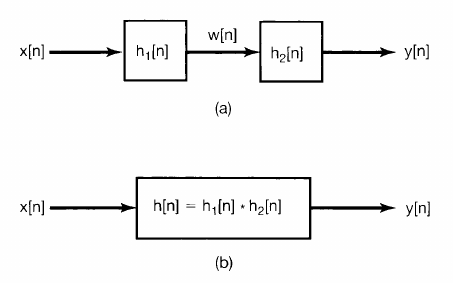
\includegraphics[width=5cm]{a45}
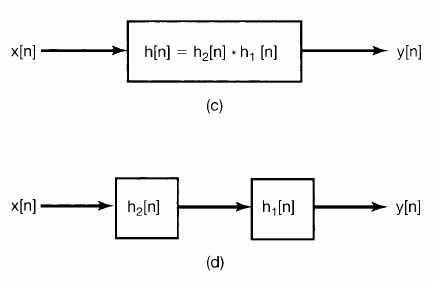
\includegraphics[width=5cm]{a46}
\end{center}
Using the associative property, we can show (a)=(b); using the commutative property we know (b)=(c), and finally 
again the associative property shows (c)=(d).\\
\vspace{1mm}\\
Consequently, the unit impulse response of a cascade of an arbitrary number of
LTI systems does not depend on the order in which they are cascaded. The same conclusions hold in continuous time.
\newpage

\section{Properties of LTI systems 2}
\textbf{Memory}\\
Recall that a system is \textit{memoryless} if its output at any time depends only on the value of the input at that same time.\\
\vspace{1mm}\\
See that the only way this can be true for a discrete-time LTI system is if $h[n]=0$ for $n\neq0$. The impulse response would be
of the form
\begin{equation*}
h[n]=K\delta[n]
\end{equation*}
Where $K=h[0]$ is a constant. (the response to each input only affects the input itself---the response at a single point is not influenced by any other points.)\\
\vspace{1mm}\\
See that the convolution sum reduces to the relation
\begin{equation*}
y[n]=Kx[n]
\end{equation*}
If a discrete-time LTI system has an impulse response $h[n]$ that is not identically zero for $n\neq0$, then the system has memory.\\
\vspace{1mm}\\
Similar properties hold for continuous-time LTI systems, which are memoryless if $h(t)=0$ for $t\neq0$. Such a memoryless LTI system has
the form
\begin{equation*}
y(t)=Kx(t)
\end{equation*}
for some constant $K$; it has the impulse response
\begin{equation*}
h(t)=K\delta(t)
\end{equation*}
Note that if $K=1$, then these systems become \textit{identity systems}, with output equal to the input and with unit response 
equal to the unit impulse. In this case, the convolution sum and integral imply that
\begin{align*}
x[n]&=x[n]*\delta[n]\\
x(t)&=x(t)*\delta(t)
\end{align*}
(next page)\newpage
\noindent\textbf{Invertibility}\\
A system is \textit{invertible} only if an \textit{inverse system} exists that, when cascaded in series with the original system, produces
an output equal to the input to the first system. Consider the following block diagrams
\begin{center}
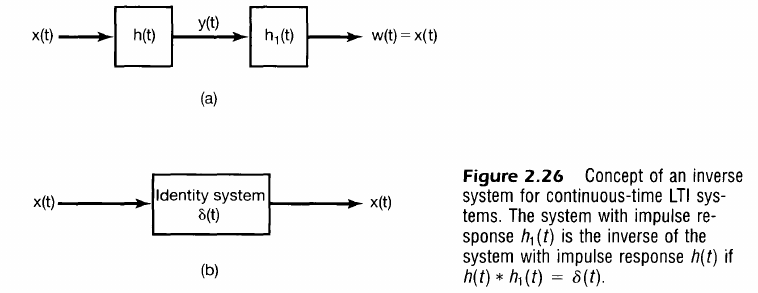
\includegraphics[width=10cm]{a47}
\end{center}
Given a system with impulse response $h(t)$, the inverse system, with impulse response $h_1(t)$, results in $w(t)=x(t)$---such that the
series interconnection is essentially identical to the identity system.\\
\vspace{1mm}\\
See (by considering associativity) that the overall impulse response
convolved with $x(t)$ is $(h(t)*h_1(t))$. As such we have a condition
that $h_1(t)$ must satisfy for it to be the impulse response of the inverse system, namely,
\begin{equation*}
h(t)*h_1(t)=\delta(t)
\end{equation*}
Similarly in discrete time, the impulse response $h_1[n]$ of the inverse system for an LTI system with impulse response $h[n]$ must
satisfy
\begin{equation*}
h[n]*h_1[n]=\delta[n]
\end{equation*}
(next page)\newpage
\noindent\textbf{Invertibility example}\\
Consider the LTI system consisting of a pure time shift
\begin{equation*}
y(t)=x(t-t_0)
\end{equation*}
Such a system is a \textit{delay} if $t_0>0$ and an \textit{advance} if $t_0<0$. If $t_0=0$, the system is the identity system and thus
is memoryless; for any other value of $t_0$, this system has memory, (since it responds to an input value at a time other than the current time).\\
\vspace{1mm}\\
By taking input equal to the $\delta(t)$ we get the impulse response
\begin{equation*}
h(t)=\delta(t-t_0)
\end{equation*}
See that as per the definition of the convolution (or by visualising the convolution)
\begin{equation*}
y(t)=x(t-t_0)=x(t)*\delta(t-t_0)
\end{equation*}
See that to invert the system, all that is required is to shift the output back. If we consider another system
\begin{equation*}
y(t)=x(t+t_0)
\end{equation*}
(see that this is just another time shift in the opposite direction) That would have the impulse response
\begin{equation*}
h_1(t)=\delta(t+t_0)
\end{equation*}
then 
\begin{equation*}
h(t)*h_1(t)=\delta(t-t_0)*\delta(t+t_0)=\delta(t)
\end{equation*}
Similarly in discrete time, a pure time shift with impulse response
$\delta[n-n_0]$ would have an inverse consisting of a time shift in the opposite direction by the same amount---another LTI system with
the impulse response $\delta[n-n_0]$.\\
(next page)\newpage
\noindent\textbf{Causality}\\
Recall the \textit{causality} property: the output of a causal system depends only on the present and past values of the input to the
system.\\
\vspace{1mm}\\
In the context of convolution, see that for a discrete-time LTI system to be causal, $y[n]$ must not depend on $x[k]$ for $k>n$, and that
in order for this to be true we must have
\begin{equation*}
h[n]=0\quad\text{for }n<0
\end{equation*}
(try to visualise the convolution to see this) This means that the impulse response of a causal LTI system must be zero before
the impulse occurs, which is consistent with the intuitive concept of causality.\\
\vspace{1mm}\\
More generally, causality for a linear system is equivalent to the condition of \textit{initial rest}: if the input to a causal system is 
0 up to some point in time, then the output must also be 0 up to that time. It is important to emphasise that the equivalence of causality
and the condition of initial rest applies only to linear systems.\\
\vspace{1mm}\\
(For example, the system $y[n]=2x[n]+3$ is not linear but is causal. However if $x[n]=0$, $y[n]=3\neq0$, so it does not satisfy
the condition of initial rest.)\\
\vspace{1mm}\\
Once again visualising the convolution sum, see that for a causal discrete-time LTI system, the $h[n]=0$ for $n<0$ implies that
it can be simplified to
\begin{equation*}
y[n]=\sum^n_{k=-\infty}x[k]h[n-k]
\end{equation*}
and the alternative equivalent form (by commutativity) becomes
(visualise as reflecting the input signal in time instead)
\begin{equation*}
y[n]=\sum^\infty_{k=0}h[k]x[n-k]
\end{equation*}
Similarly, a continuous-time LTI system is causal if
\begin{equation*}
h(t)=0\quad\text{for }t<0
\end{equation*}
where the convolution integral is given by
\begin{equation*}
y(t)=\int^t_{-\infty}x(\tau)h(t-\tau)d\tau=\int^\infty_0h(\tau)x(t-\tau)d\tau
\end{equation*}
While causality is a property of systems, it is common terminology to refer to a signal as being causal if it is zero for $n<0$ or $t<0$. 
The motivation for this comes from the conditions for causality as defined above: Causality for an LTI system is equivalent to its
impulse response being a `causal' signal.\\
(next page)\newpage
\noindent\textbf{Stability}\\
Recall that a system is \textit{stable} if every bounded input produces a bounded output. We want to derive a condition to determine
whether a candidate LTI system is stable; consider an input $x[n]$ that is bounded in magnitude:
\begin{equation*}
x[n]<B\quad\text{for all }n
\end{equation*}
Suppose we apply this input to an LTI system with unit impulse response $h[n]$. Then, using the convolution sum, we obtain an expression
for the \textit{magnitude} of the output as
\begin{equation*}
|y[n]|=\left|\sum^{+\infty}_{k=-\infty}h[k]x[n-k]\right|
\end{equation*}
Since the magnitude of the sum of a set of numbers is no larger than the sum of the magnitudes of the numbers, it follows that
\begin{equation*}
|y[n]|\leq\sum^{+\infty}_{k=-\infty}|h[k]||x[n-k]|
\end{equation*}
We know that $|x[n-k]|<B$ for all values of $k$ and $n$. This implies that
\begin{equation*}
|y[n]|\leq B\sum^{+\infty}_{k=-\infty}|h[k]|\quad\text{for all }n
\end{equation*}
We conclude that the impulse response is \textit{absolutely summable} if
\begin{equation*}
\sum^{+\infty}_{k=-\infty}|h[k]|<\infty
\end{equation*}
See that if the impulse response is absolutely summable, $y[n]$ will be bounded in magnitude, and hence the system is stable. This means
that the above is a sufficient condition to gaurantee the stability of a discrete-time LTI system. (see that this condition 
is also necessary, as if it were not satisfied then there would be unbounded outputs)\\
(next page)\newpage
\noindent\textbf{Stability cont.}\\
In continuous time we have an analagous characterisation of stabilityin terms of the impulse response of an LTI system; 
if $|x(t)|<B$ for all $t$, then it follows that
\begin{align*}
|y(t)|&=\left|\int^{+\infty}_{-\infty}h(\tau)x(t-\tau)d\tau\right|\\
&\leq\int^{+\infty}_{-\infty}|h(\tau)||x(t-\tau)|d\tau\\
&\leq B\int^{+\infty}_{-\infty}|h(\tau)|d\tau
\end{align*}
Therefore, the system is stable if it is \textit{absolutely integrable}:
\begin{equation*}
\int^{+\infty}_{-\infty}|h(\tau)|d\tau<\infty
\end{equation*}
As with the discrete case this is actually a necessary condition for stability, as if it were unsatisfied, it would lead to unbounded 
outputs.\\
\vspace{1mm}\\
\textbf{Stability example 1---stable}\\
Consider a system that is a pure time shift in either continuous or discrete time. Then in discrete time 
\begin{equation*}
\sum^{+\infty}_{n=-\infty}|h[n]|=
\sum^{+\infty}_{n=-\infty}|\delta[n-n_0]|=1
\end{equation*}
while in continuous time
\begin{equation*}
\int^{+\infty}_{-\infty}|h(\tau)|d\tau=
\int^{+\infty}_{-\infty}|\delta(\tau-t_0)|d\tau=1
\end{equation*}
and we can conclude both systems are stable.\\
(next page)\newpage
\noindent\textbf{Stability example 2---unstable}\\
Consider now the accumulator, with an impulse response equal to $u[n]$; see that the impulse response in this case is not absolutely
summable:
\begin{equation*}
\sum^{\infty}_{n=-\infty}|u[n]|=\sum^{\infty}_{n=0}u[n]=\infty
\end{equation*}
Similarly consider the integrator (the continuous-tiem counterpart of the accumulator):
\begin{equation*}
y(t)=\int^t_{-\infty}x(\tau)d\tau
\end{equation*}
This is also an unstable system; see that the impulse response for the integrator is:
\begin{equation*}
h(t)=\int^t_{-\infty}\delta(\tau)d\tau=u(t)
\end{equation*}
and 
\begin{equation*}
\int^{+\infty}_{-\infty}|u(t)|d\tau=\int^{+\infty}_0|u(t)|d\tau=\infty
\end{equation*}
Since the impulse response is not absolutely integrable, the system is not stable.
\newpage

\section{The Unit Step Response of an LTI system}
There is another signal that is also used quite often in describing the behaviour of LTI systems: the \textit{unit step response} $s[n]$
or $s(t)$; as implied, it corresponds to the output when $x[n]=u[n]$ or $x(t)=u(t)$.\\
\vspace{1mm}\\
 From the convolution-sum representation, see that
the step response can be found by convolution of the unit step with the impulse response:
\begin{equation*}
s[n]=u[n]*h[n]
\end{equation*}
Also see that by commutativity, $s[n]=h[n]*u[n]$, and therefore $s[n]$ can be viewed as the response to the input $h[n]$ of a 
discrete-time LTI system with unit response $u[n]$. Since $u[n]$ is the unit impulse response of the \textit{accumulator},
this means that an input $h[n]$ to an accumulator yields the unit step response:
\begin{equation*}
s[n]=\sum^n_{k=-\infty}h[k]
\end{equation*}
The fact that we know the inverse system for the accumulator means we know then that $h[n]$ can be recovered from $s[n]$ using the
relation
\begin{equation*}
h[n]=s[n]-s[n-1]
\end{equation*}
That is, the step response of a discrete-time LTI system is the \textit{running sum of its impulse response} (try to visualise this!). 
Conversely, the impulse response of a discrete-time LTI system is the first difference of its step response.\\
\vspace{1mm}\\
Similarly in continuous time, the step response of an LTI system with impulse response $h(t)$ is given by $s(t)=u(t)*h(t)=h(t)*u(t)$.
The \textit{integrator} has $u(t)$ as its impulse response, so this is equivalent to inputting $h(t)$ into an integrator:
\begin{equation*}
s(t)=\int^t_{-\infty}h(\tau)d\tau
\end{equation*}
as such see that the unit impulse response can be recovered as the first derivative
\begin{equation*}
h(t)=\frac{ds(t)}{dt}=s'(t)
\end{equation*}
The unit step response of a continuous-time LTI system is the running integral of its impulse response, and the unit impulse response is
the first derivative of the unit step response.\\
\vspace{1mm}\\
In that sense, the unit step response can also be used to characterise an LTI system, since we can calculate the unit impulse response
from it.
\newpage

\section{Causal LTI systems described by differential and difference equations}
\textbf{Linear constant-coefficient differential equations}\\
An important point about differential equations is that they provide an \textit{implicit} specification of a system. That is, they
describe a relationship between the input and the output, rather than an \textit{explicit} expression for the system output as a 
function of the input. (meaning they don't immediately tell you the output from a given input value, unlike say a function)\\
\vspace{1mm}\\
\textbf{Auxiliary conditions---Initial rest}\\
Recall that the formation of an explicit solution to a differential equation requires the specification of certain 
\textit{auxiliary/initial conditions} in order to fully evaluate the \textit{homogeneous solution} or the 
\textit{natural response} of the system. Also 
recall that different choices of auxiliary conditions will lead to different relationships between the input and output.\\
\vspace{1mm}\\
In some cases this auxiliary contition might take the form of the condition of \textit{initial rest}, where if $x(t)=0$ for 
$t<t_0$, then $y(t)$ must also equal 0 for $t<t_0$. It is important to emphasise that a condition of initial rest does not 
specify a zero initial condition at a fixed point in time, but rather adjusts this point in time so that the \textit{response is zero 
until the input becomes nonzero}. (thus, if $x(t)=0$ for $t\leq t_0$, then we could use $y(t_0)=0$ to solve for the output for $t>t_0$)\\
(next page)\newpage
\noindent\textbf{General form}\\
A general $N$th-order linear constant-coefficient differential equation is given by
\begin{equation*}
\sum^N_{k=0}a_k\frac{d^ky(t)}{dt^k}=\sum^M_{k=0}b_k\frac{d^kx(t)}{dt^k}
\end{equation*}
The \textit{order} refers to the highest derivative of the output $y(t)$ appearing in the equation. In the case where $N=0$, 
see that this reduces to
\begin{equation*}
y(t)=\frac{1}{a_0}\sum^M_{k=0}b_k\frac{d^kx(t)}{dt^k}
\end{equation*}
In this case, $y(t)$ is an explicit function of the input $x(t)$ and its derivatives. 
For $N\geq1$, the equation would specify an implicit relationship in terms of the input. In this case, the analysis of the equation would 
proceed in a way analagous to that of a first-order DE, with a solution consisting of two parts---a particular solution plus a solution to
the homogeneous differential equation
\begin{equation*}
\sum^N_{k=0}a_k\frac{d^ky(t)}{dt^k}=0
\end{equation*}
As in the first-order case, the general form does not completely specify the output in terms of the input, and we need to identify 
auxiliary conditions to determine completely the input-output relationship for the system. Should we consider initial rest, we assume then
that if $x(t)=0$ for $t\leq t_0$, then $y(t)=0$ for $t\leq t_0$, and therefore, the response for $t>t_0$ can be calculated with the 
initial conditions
\begin{equation*}
y(t_0)=\frac{dy(t_0)}{dt}=\ldots=\frac{d^{N-1}y(t_0)}{dt^{N-1}}=0
\end{equation*}
(For an $N$th order DE we'll need $N$ initial conditions. This comes from the fact that the characteristic polynomial will have $N$ roots,
so $N$ exponentials where any linear combination of them would satisfy the homogeneous equation, thus warranting the need for the initial conditions
to determine the coefficients of this linear combination.)\\
\vspace{1mm}\\
Under the condition of initial rest, the system described in the general form above is causal and LTI.\\
(next page)\newpage
\noindent\textbf{Linear constant-coefficient difference equations---General form}\\
The discrete-time counterpart of the previous general form is the $N$th-order linear constant-coefficient difference equation
\begin{equation*}
\sum^N_{k=0}a_ky[n-k]=\sum^M_{k=0}b_kx[n-k]
\end{equation*}
All equations of this type can be solved in a manner analagous to that for differential equations. As before, the solution 
$y[n]$ can be written as the sum of a particular solution to the above plus a solution to the homogeneous equation
\begin{equation*}
\sum^N_{k=0}a_ky[n-k]=0
\end{equation*}
As in the continuous-time case, the general form is not sufficient to completely specify an output, and requires specification of
auxiliary conditions (in this case this might be $y[n-1],\ldots y[n-N]$). 
The condition of initial rest can also be applied here, where if $x[n]=0$ for $n<n_0$, then $y[n]=0$ for $n<n_0$
as well. With initial rest, the system would be LTI and causal.\\
\vspace{1mm}\\
\textbf{Recursive equations}\\
Although all of these properties can be developed following an approach that directly parallels those for differential equations, the
discrete-time case offers an alternative path. See that the general form can be rearranged as
\begin{equation*}
y[n]=\frac{1}{a_0}\left\{\sum^M_{k=0}b_kx[n-k]-\sum^N_{k=1}a_ky[n-k]\right\}
\end{equation*}
See that the output at time $n$ can be expressed in terms of previous values of the input and output. An equation of this form is called 
a \textit{recursive equation}, since it specifies a recursive procedure for determining the output in terms of the input and previous
outputs. In the special case where $N=0$, this reduces to
\begin{equation*}
y[n]=\sum^M_{k=0}\frac{b_k}{a_0}x[n-k]
\end{equation*}
Here $y[n]$ is an explicit function of the present and previous values of the input. For that reason this is often called a
\textit{nonrecursive equation} (since we do not recursively use previously computed values to compute the present output).\\
\vspace{1mm}\\
Although we do not require auxiliary conditions for the case of $N=0$, such conditions are needed for the recursive case when $N\geq1$.\\
(next page)\newpage
\noindent\textbf{Difference equation example}\\
Consider the difference equation
\begin{equation*}
y[n]-\frac{1}{2}y[n-1]=x[n]
\end{equation*}
rewritten as
\begin{equation*}
y[n]=x[n]+\frac{1}{2}y[n-1]
\end{equation*}
this highlights the idea that we need the previous value of the output, $y[n-1]$, to calculate the current value. Thus to begin the
recursion we need an initial condition.\\
\vspace{1mm}\\
Suppose we impose the condition of initial rest and consider the input
\begin{equation*}
x[n]=K\delta[n]
\end{equation*}
In this case, since $x[n]=0$ for $n\leq-1$ (because of the delta function), the condition of initial rest implies that $y[n]=0$ for
$n\leq-1$, so we have as an initial condition $y[-1]=0$. Starting from the initial condition, see that we can recursively solve
for successive values of $y[n]$ for $n\geq0$ as follows:
\begin{align*}
y[0]&=x[0]+\frac{1}{2}y[-1]=K\\
y[1]&=x[1]+\frac{1}{2}y[0]=\frac{1}{2}K\\
y[2]&=x[2]+\frac{1}{2}y[1]=\left(\frac{1}{2}\right)^2K\\
\vdots&\\
y[n]&=x[n]+\frac{1}{2}y[n-1]=\left(\frac{1}{2}\right)^nK
\end{align*}
See additionally that by setting $K=1$ we obtain the impulse response for the system as
\begin{equation*}
h[n]=\left(\frac{1}{2}\right)^nu[n]
\end{equation*}
(see that some initial conditions may lead to a non-LTI system, in which obtaining the impulse response be much less useful)
\newpage

\section{Block diagram representations of first-order systems described by differential and difference equations}









\appendix
\chapter{Other proofs}
\section{Sum of geometric series}
Here we show
\begin{equation*}
S_n=\sum^{n-1}_{i=0}\alpha^i=\frac{\alpha^n-1}{\alpha-1}
\end{equation*}
This can be seen from
\begin{align*}
(\alpha-1)S_n&=\alpha\sum^{n-1}_{i=0}\alpha^i-\sum^{n-1}_{i=0}\alpha^i\\
&=\sum^{n}_{i=1}\alpha^i-\sum^{n-1}_{i=0}\alpha^i\\
&=\alpha^n+\sum^{n-1}_{i=1}\alpha^i-(1+\sum^{n-1}_{i=1}\alpha^i)\\
&=\alpha^n-1
\end{align*}
and so
\begin{equation*}
S_n=\frac{\alpha^n-1}{\alpha-1}
\end{equation*}






\end{document}
